% Draft for Journal of Mathematical Philosophy (double-anonymous submission).
% Requires cm-super: the T1-encoded sans headings fall back to bitmap
% Type 3 fonts without it.
\documentclass[11pt,a4paper]{article}

% ── Page & type ──────────────────────────────────────────────
\usepackage[margin=1.15in,headheight=22pt]{geometry}
\usepackage[T1]{fontenc}
\usepackage{mathpazo}
\usepackage[expansion=false]{microtype}
\usepackage{setspace}
\setstretch{1.12}
\raggedbottom
% Long monospace declaration names leave some lines unbreakable at
% default tolerances; emergency stretch engages only when line
% breaking would otherwise fail.
\setlength{\emergencystretch}{1.5em}

% ── Colour (restrained ink; anonymous journal look) ──────────
\usepackage{xcolor}
\definecolor{ink}{HTML}{1A1A1A}
\definecolor{muted}{HTML}{5A5A5A}
\definecolor{rule}{HTML}{C8C4BC}
\definecolor{accent}{HTML}{2C3E50}
\definecolor{soft}{HTML}{F4F1EC}
\definecolor{nodefill}{HTML}{F7F5F1}
\definecolor{openbg}{HTML}{F7F5F1}
\definecolor{refusedbg}{HTML}{F3EEEA}
\definecolor{philbg}{HTML}{EEF2F5}
\color{ink}

% ── Math, theorems, lists ────────────────────────────────────
\usepackage{amsmath,amssymb,amsthm}
\usepackage{mathtools}
\usepackage{enumitem}
\setlist[enumerate]{leftmargin=*,itemsep=0.2em,topsep=0.35em}
\setlist[itemize]{leftmargin=*,itemsep=0.15em,topsep=0.3em}

\theoremstyle{plain}
\newtheorem{theorem}{Theorem}[section]
\newtheorem{proposition}[theorem]{Proposition}
\newtheorem{lemma}[theorem]{Lemma}
\newtheorem{corollary}[theorem]{Corollary}
\theoremstyle{definition}
\newtheorem{definition}[theorem]{Definition}
\theoremstyle{remark}
\newtheorem{remark}[theorem]{Remark}
\newtheorem{interpretation}[theorem]{Interpretation}

% ── Graphics & layout ────────────────────────────────────────
\usepackage{booktabs}
\usepackage{tabularx}
\usepackage{graphicx}
\usepackage{tikz}
\usetikzlibrary{arrows.meta,positioning,calc,fit}
\usepackage[skins,breakable]{tcolorbox}
\usepackage{titlesec}
\usepackage{fancyhdr}
\usepackage{caption}
\usepackage{needspace}
\usepackage[hidelinks]{hyperref}
\captionsetup{font=small, labelfont={sf,bf}, textfont=it, skip=0.45em}

\titleformat{\section}
  {\large\bfseries\color{accent}\sffamily}
  {\thesection}{0.6em}{}
  [\vspace{-0.35em}{\color{rule}\titlerule[0.5pt]}]
\titleformat{\subsection}
  {\normalsize\bfseries\color{accent}\sffamily}
  {\thesubsection}{0.5em}{}
\titlespacing*{\section}{0pt}{1.35em}{0.55em}
\titlespacing*{\subsection}{0pt}{0.95em}{0.35em}

\pagestyle{fancy}
\fancyhf{}
\renewcommand{\headrulewidth}{0.4pt}
\renewcommand{\headrule}{\hbox to\headwidth{\color{rule}\leaders\hrule height \headrulewidth\hfill}}
\fancyhead[L]{\color{muted}\scriptsize Classification of self-actions}
\fancyhead[R]{\color{muted}\scriptsize Unique involutive survivor}
\fancyfoot[C]{\color{muted}\small\thepage}
\fancypagestyle{plain}{%
  \fancyhf{}%
  \renewcommand{\headrulewidth}{0pt}%
  \fancyfoot[C]{\color{muted}\small\thepage}%
}

% Status callouts (open / refused / philosophical)
\newtcolorbox{statusopen}{
  breakable, colback=openbg, colframe=rule, boxrule=0.5pt,
  borderline west={2.2pt}{0pt}{accent},
  arc=1pt, left=10pt, right=10pt, top=7pt, bottom=7pt,
  before skip=0.7em, after skip=0.7em,
  title={\sffamily\bfseries Open},
  fonttitle=\small\sffamily, coltitle=accent, colbacktitle=soft,
  attach boxed title to top left={yshift=-2mm,xshift=8pt},
  boxed title style={colframe=rule, boxrule=0.4pt, arc=1pt,
    left=5pt,right=5pt,top=1pt,bottom=1pt}
}
\newtcolorbox{statusrefused}{
  breakable, colback=refusedbg, colframe=rule, boxrule=0.5pt,
  borderline west={2.2pt}{0pt}{accent},
  arc=1pt, left=10pt, right=10pt, top=7pt, bottom=7pt,
  before skip=0.7em, after skip=0.7em,
  title={\sffamily\bfseries Refused},
  fonttitle=\small\sffamily, coltitle=accent, colbacktitle=soft,
  attach boxed title to top left={yshift=-2mm,xshift=8pt},
  boxed title style={colframe=rule, boxrule=0.4pt, arc=1pt,
    left=5pt,right=5pt,top=1pt,bottom=1pt}
}
\newtcolorbox{statusphil}{
  breakable, colback=philbg, colframe=rule, boxrule=0.5pt,
  borderline west={2.2pt}{0pt}{accent},
  arc=1pt, left=10pt, right=10pt, top=7pt, bottom=7pt,
  before skip=0.7em, after skip=0.7em,
  title={\sffamily\bfseries Philosophical},
  fonttitle=\small\sffamily, coltitle=accent, colbacktitle=soft,
  attach boxed title to top left={yshift=-2mm,xshift=8pt},
  boxed title style={colframe=rule, boxrule=0.4pt, arc=1pt,
    left=5pt,right=5pt,top=1pt,bottom=1pt}
}

\newcommand{\Fund}{\mathsf{Fund}}
\newcommand{\Bool}{\mathsf{Bool}}
\newcommand{\comp}{\circ}
\newcommand{\Ztwo}{\mathbb{Z}/2\mathbb{Z}}
\newcommand{\act}{a}
\newcommand{\dep}[1]{%
  \par\noindent{\small\color{muted}\sffamily Dependence:}~\textit{#1}\par\medskip}

\title{Classification of Self-Actions\\[0.25em]
  and the Unique Involutive Survivor}
\author{} % anonymized for double-anonymous review
\date{}

\begin{document}
\maketitle

\begin{abstract}
We present two eliminative classifications over one kernel. The first
classifies self-actions $a:\alpha\to\alpha$ by local orbit shape. Rest,
asymmetric step, and erasure each meet a formal obstruction in the ambient
of pointed symmetric steps; the surviving shape is the fixed-point-free
two-cycle. That survivor is characterised by a universal property:
$(\Bool,\neg)$ is initial among pointed unoriented acts, and every
fundamental act reads as negation. From fundamentality we obtain a
Lawvere-style seal with quantitative grain (names lag predicates at every
level, and the lag recedes under completion), an $\omega$-ladder of namers
whose colimit is duration, and, after transferring losslessness to forward
microsteps by two-bounce factorisation, registration, capacity, and a
single $\Ztwo$-underdetermination with three faces. Canonicity of the
two-bounce pair fails; channel \emph{swap} nevertheless covers step
reversal, and content gauges are separated from packaging gauges so that
factorisation non-uniqueness does not inflate the dictionary $\Ztwo$. The
second classification repeats the eliminative method on motion: among
second-order nearest-neighbour updates over the same kernel, losslessness
forces the xor form, and parity, pole invariance, and a drawing condition
leave exactly one coupling up to pointwise flip, whose dynamics is the
discrete wave step. A carrier-size dichotomy places the residual flip:
on carriers divisible by four it is packaging, realised by an explicit
conjugating mask, and on every other carrier no equivariant
identification of the two dynamics exists, so there the flip carries
content. The classified dynamics factors into two involutions
definitionally, reverses by swapping them, carries a period spectrum
governed by a gcd law, and returns within capacity. At the edge of the
ladder the complete gauge histories form a boundary: every rung embeds
there with effective separation, the seal persists at the boundary's own
carrier, and the exclusion of erasure fails, so losslessness is a
finite-stage law whose failure at the colimit is itself a theorem. On
this base we assemble a conditional monist package,
\emph{self-articulation}: a registered denial of one drawn distinction
draws the registering carrier (retorsion); a drawn distinction forces the
live involutive reading; witnesses arise as ladder inhabitants; every
presentation of the canon to a second term retracts the canon's own
articulation; and completeness exists only as duration. The dictionary
carries two worked exhibits: a certificate for the meta-problem of
consciousness, deriving the report structure of the explanatory gap while
refusing all qualia claims, and a certificate identifying the classified
dynamics with reversible lattice computation. The development is
machine-checked in Lean~4 (no Mathlib, no $\mathtt{sorry}$).
\end{abstract}

\noindent{\sffamily\bfseries\color{accent} Keywords.}
classification; involution; universal property; Lawvere diagonal;
wave dynamics; reversible computation; self-articulation; retorsion;
meta-problem; underdetermination; gauge; machine-checked mathematics.

\section{Introduction}
\label{sec:intro}

The central contribution of this paper is a twofold eliminative
classification: the kernel is forced, and its motion is forced. The
static half classifies self-actions. Given $a:\alpha\to\alpha$, the local
possibilities at a state are rest, two-cycle, asymmetric step, and---as a
pairwise defect---erasure. In a precisely specified ambient, every shape
except one encounters an obstruction. The survivor is the live two-cycle.
Negation on $\Bool$~\cite{bool} is not assumed at the outset; it is the
unique object (up to label swap) satisfying the universal property, in
the standard categorical sense~\cite{maclane}, of that survivor.

The dynamic half repeats the same eliminative method one level up, on
the equation of motion. Among second-order nearest-neighbour updates
over the kernel, the demand that no two histories merge forces the
update into an xor form, and three ambient conditions that mirror the
static ones (parity, pole invariance, and a drawing condition) leave
exactly one coupling up to pointwise flip. The survivor's dynamics is
the discrete wave step: it factors into two involutions definitionally,
it reverses by swapping them, its period spectrum obeys a gcd law and is
reshaped by boundary conditions alone, and every state returns within
the capacity of its carrier. Motion is thereby classified with the same
discipline as the kernel, and no equation of motion is chosen by hand.

A further contribution assembles, on that base, a conditional monist
package. Given one drawn distinction, articulation as negation is
forced, witnesses arise only as inhabitants of the resulting ladder, no
presentation of the canon to a second term carries content beyond the
canon's own articulation, and completeness exists only as the colimit of
ascent. The package is a single machine-checked conjunction
(Theorem~\ref{thm:selfart}); its identification with worldhood is
confined to a marked interpretation, and the dictionary works two
certificates, one for the meta-problem of consciousness and one
identifying the classified dynamics with reversible lattice
computation.

The formal development then follows a fixed dependency:

\begin{center}
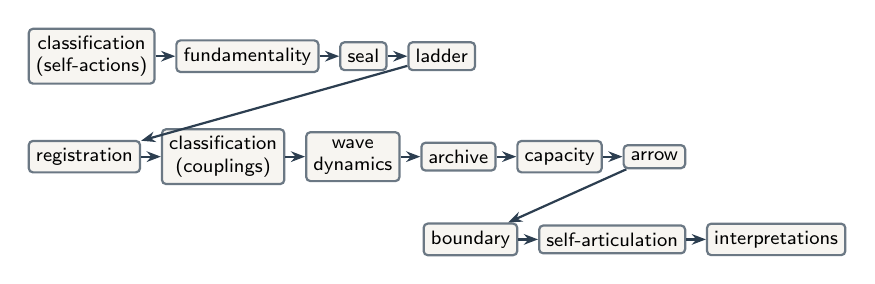
\begin{tikzpicture}[
  font=\scriptsize\sffamily,
  N/.style={draw=accent!70, fill=nodefill, thick, rounded corners=1.5pt,
    inner sep=2.6pt, align=center},
  arr/.style={-{Stealth[length=1.8mm]}, accent, thick}
]
  \node[N] (c) {classification\\(self-actions)};
  \node[N, right=2.5mm of c] (f) {fundamentality};
  \node[N, right=2.5mm of f] (s) {seal};
  \node[N, right=2.5mm of s] (l) {ladder};
  \node[N, below=7mm of c.south west, anchor=north west] (r) {registration};
  \node[N, right=2.5mm of r] (c2) {classification\\(couplings)};
  \node[N, right=2.5mm of c2] (wv) {wave\\dynamics};
  \node[N, right=2.5mm of wv] (a) {archive};
  \node[N, right=2.5mm of a] (k) {capacity};
  \node[N, right=2.5mm of k] (w) {arrow};
  \node[N, below=7mm of w.south east, anchor=north east] (sa) {self-articulation};
  \node[N, left=2.5mm of sa] (bd) {boundary};
  \node[N, right=2.5mm of sa] (i) {interpretations};
  \draw[arr] (c) -- (f);
  \draw[arr] (f) -- (s);
  \draw[arr] (s) -- (l);
  \draw[arr] (l) -- (r);
  \draw[arr] (r) -- (c2);
  \draw[arr] (c2) -- (wv);
  \draw[arr] (wv) -- (a);
  \draw[arr] (a) -- (k);
  \draw[arr] (k) -- (w);
  \draw[arr] (w) -- (bd);
  \draw[arr] (bd) -- (sa);
  \draw[arr] (sa) -- (i);
\end{tikzpicture}
\end{center}
Each arrow is a theorem or a defined interface; the second
classification node feeds the dynamics row, and philosophical commentary
is postponed until the supporting machinery is in place.

\paragraph{Method and layers.}
The text maintains three layers.
\begin{enumerate}[label=(\arabic*)]
\item \textbf{Formal mathematics} --- definitions, theorems, proofs.
\item \textbf{Philosophical interpretation} --- what the mathematics
suggests, marked as such.
\item \textbf{Dictionary} --- optional physical or contemplative
identifications, admitted only by certificate.
\end{enumerate}
Claims are tagged by status: proved, corollary, interpretation, open,
refused, or philosophical residue. Residue is reduced by
reclassification: items become theorems, audited residues at the base,
or certificate data (Section~\ref{sec:status}). The companion Lean~4 corpus~\cite{lean4}
(no Mathlib~\cite{mathlib}, no $\mathtt{sorry}$) supplies declaration
names; this paper is
self-contained at the level of statements.

\paragraph{Roadmap.}
Section~\ref{sec:arch} gives the architecture.
Sections~\ref{sec:class}--\ref{sec:fund} carry out the static
classification and the universal characterisation of the survivor.
Sections~\ref{sec:seal}--\ref{sec:ladder} obtain seal and ladder.
Section~\ref{sec:reg} transfers losslessness by two-bounce
factorisation.
Section~\ref{sec:coupling} carries out the dynamic classification, and
Section~\ref{sec:wave} develops the classified wave dynamics.
Sections~\ref{sec:archive}--\ref{sec:arrow} record registration
consequences, capacity, and the arrow as address.
Section~\ref{sec:z2} states the single $\Ztwo$, the gauge demarcation,
and the placement of the coupling flip.
Section~\ref{sec:boundary} presents the boundary of complete gauge
histories and the edge failure of losslessness.
Section~\ref{sec:selfart} assembles the self-articulation package and
sorts its admissible readings.
Section~\ref{sec:dict} confines the dictionary to two worked
certificates.
Section~\ref{sec:status} collects open, refused, and philosophical items.
Section~\ref{sec:related} situates the development in prior work.
Section~\ref{sec:concl} concludes.


\section{Architecture}
\label{sec:arch}

The companion corpus is stratified into three layers with downward-only
imports (Figure~\ref{fig:layers}).

\begin{figure}[ht]
\centering
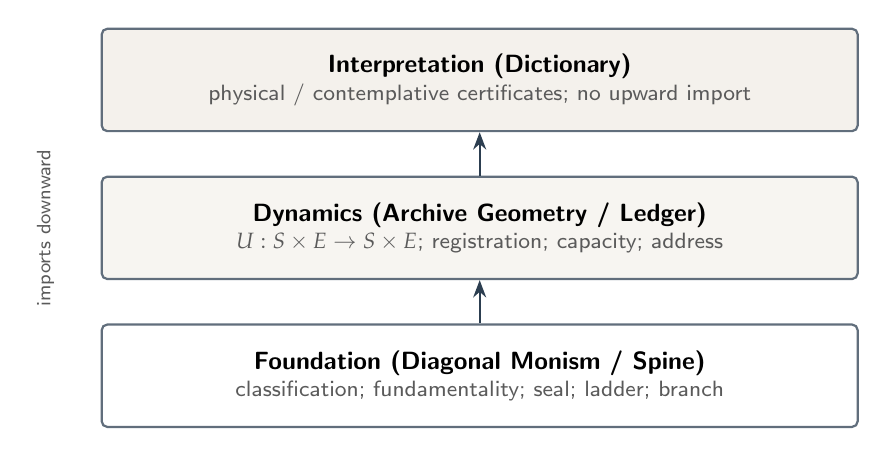
\begin{tikzpicture}[
  font=\small\sffamily,
  layer/.style={draw=accent!75, thick, rounded corners=2pt, minimum width=96mm,
    minimum height=13mm, align=center, inner sep=4pt, fill=nodefill},
  arr/.style={-{Stealth[length=2.2mm]}, accent, thick}
]
\node[layer, fill=soft] (dict) {%
  \textbf{Interpretation (Dictionary)}\\[-1pt]
  {\footnotesize\color{muted} physical / contemplative certificates; no upward import}};
\node[layer, below=5.5mm of dict] (led) {%
  \textbf{Dynamics (Archive Geometry / Ledger)}\\[-1pt]
  {\footnotesize\color{muted} $U:S\times E\to S\times E$; registration; capacity; address}};
\node[layer, fill=white, below=5.5mm of led] (sp) {%
  \textbf{Foundation (Diagonal Monism / Spine)}\\[-1pt]
  {\footnotesize\color{muted} classification; fundamentality; seal; ladder; branch}};
\draw[arr] (sp) -- (led);
\draw[arr] (led) -- (dict);
\node[muted, font=\scriptsize\sffamily, rotate=90] at ($(sp.west)!0.5!(dict.west)+(-7mm,0)$)
  {imports downward};
\end{tikzpicture}
\caption{Three-layer architecture. Arrows indicate permitted dependence
(foundation supports dynamics; dynamics support interpretation). The
figure orients the reader; it proves nothing.}
\label{fig:layers}
\end{figure}

\noindent
Within the foundation, the dependency is
classification~$\to$~fundamentality~$\to$~seal~$\to$~ladder.
The dynamics layer imports losslessness along an interface
(registration via two-bounce), classifies the couplings and develops the
resulting wave dynamics, realises archive and capacity on the ladder
carrier, and exports address as the arrow reading. The dictionary
layer consumes those exports; it does not feed them.

The companion corpus realises the three layers as four build packages:
a spine package (foundation); a ledger package and a bridge package
jointly constituting the dynamics layer, the bridge holding the
interface theorems that import both spine and ledger together with the
dynamics arc of Sections~\ref{sec:coupling}--\ref{sec:wave}
(modules \texttt{DynamicsAmbient}, \texttt{WaveDynamics},
\texttt{PeriodSpectrum}, \texttt{Recurrence}); and a dictionary
package with exhibits (interpretation). Imports remain downward
throughout. A fifth package, \texttt{formal/experimental}, is
quarantined by construction: no spine, ledger, bridge, or dictionary
module imports it, and the annex at the end of the paper inventories
what it holds. Citations at that package occur in exactly two places,
the boundary results of Section~\ref{sec:boundary} and the
coupling-flip placement of Section~\ref{sec:z2}, and they are flagged
as such where they appear. A few dynamics-layer
declarations bear physically suggestive names as mnemonics for
combinatorial statements; the names import no identification, which
remains certificate-only (Section~\ref{sec:dict}).


\section{Classification of self-actions}
\label{sec:class}

\begin{definition}[Arena data]
\label{def:arena}
Fix a type $\alpha$ and a map $a:\alpha\to\alpha$. Write
\[
  \mathsf{Step}(a)(x,y)\ :\Leftrightarrow\ y=a(x).
\]
Call $a$ a \emph{symmetric step} when $\mathsf{Step}(a)$ is a symmetric
relation; equivalently, $a\comp a=\mathrm{id}$. Call $a$ \emph{live}
when $\forall x.\, a(x)\neq x$. Call $a$ \emph{lossless} when $a$ is
injective. Call $a$ \emph{erasing} when distinct states share a
successor.
\end{definition}

\begin{theorem}[Pointwise classification]
\label{thm:class}
For decidable equality on $\alpha$, at each $z$ exactly one of the
following holds: (i)~rest ($a(z)=z$), with all iterates stagnant;
(ii)~two-cycle at $z$ ($a(z)\neq z$ and $a(a(z))=z$), with every iterate
equal to $z$ or $a(z)$; (iii)~asymmetric step at $z$ ($a(a(z))\neq z$).
The three cases are pairwise incompatible. Erasure is diagnosed
separately as a pairwise defect of losslessness.
\end{theorem}

\begin{center}
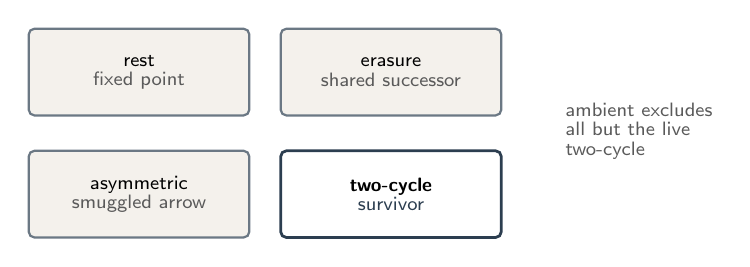
\begin{tikzpicture}[
  font=\scriptsize\sffamily,
  box/.style={draw=accent!70, fill=nodefill, thick, rounded corners=2pt,
    minimum width=28mm, minimum height=11mm, align=center},
  kill/.style={box, fill=soft},
  live/.style={box, fill=white, draw=accent, line width=1pt}
]
  \node[kill] (r) at (0,0) {rest\\[-1pt]{\color{muted}fixed point}};
  \node[kill] (e) at (3.2,0) {erasure\\[-1pt]{\color{muted}shared successor}};
  \node[kill] (a) at (0,-1.55) {asymmetric\\[-1pt]{\color{muted}smuggled arrow}};
  \node[live] (t) at (3.2,-1.55) {\textbf{two-cycle}\\[-1pt]{\color{accent}survivor}};
  \node[muted, font=\scriptsize\sffamily, align=left] at (6.35,-0.75)
    {ambient excludes\\[-1pt]all but the live\\[-1pt]two-cycle};
\end{tikzpicture}
\end{center}

\begin{remark}[Status]
Theorem~\ref{thm:class} is proved. It is the eliminative engine of the
paper: subsequent sections impose ambient constraints under which (i)
and (iii), and erasure, are excluded as candidates for fundamentality.
\end{remark}

Symmetric step is the ambient equation used below. It jointly excludes
asymmetric arrow (case~(iii) globally) and, by the next corollary,
erasure.

\begin{proposition}[In-arena losslessness]
\label{prop:no-erase}
If $a$ is a symmetric step, then $a$ is not erasing.
\end{proposition}

\begin{remark}[Status]
Corollary of Definition~\ref{def:arena} (involution $\Rightarrow$
injectivity). Not an independent creed.
\end{remark}

\begin{theorem}[Ambient uniqueness, one-variable equational fragment]
\label{thm:ambient-unique}
Relative to the arena signature of Definition~\ref{def:arena} (one type,
one endomap), every single equation in one free variable has the form
$a^{m}(x)=a^{n}(x)$. Among those equations:
\begin{enumerate}[label=(\roman*)]
\item $a^{m}=a^{n}$ with $n\ge 1$ need not force injectivity
($a^{2}=a$ admits erasure);
\item $a^{m}=\mathrm{id}$ forces losslessness; $m=1$ is rest; for every
$m\ge 3$ an $m$-cycle is a countermodel with an asymmetric point;
\item hence $a^{2}=\mathrm{id}$ is the unique nontrivial one-variable
single equation that excludes both smuggled arrow and smuggled loss.
\end{enumerate}
\end{theorem}

\begin{remark}[Status]
Proved by exhaustive classification of one-variable equations relative to
the signature, with finite countermodels (including the $m$-cycle family
for all $m\ge 3$). Multi-variable single equations over the same
signature---for example $\forall x\,\forall y.\,a(x)=a(y)$---force
constancy on the image and are erasing on any carrier with two or more
points, so they die immediately as ambients for fundamentality.
Ambients beyond the one-variable equational fragment are refused by
parsimony of the arena language (Section~\ref{sec:status}).
Interpretation~\ref{int:ambient} records only the residual choice of
signature itself.
\end{remark}

\begin{interpretation}
\label{int:ambient}
Symmetric step is not an arbitrary modelling confession: by
Theorem~\ref{thm:ambient-unique} it is the unique nontrivial
one-variable single-equation ambient in the arena signature that bans
smuggled time and smuggled loss. What remains is the signature
declaration of Definition~\ref{def:arena}---one type, one
endomap---stated in daylight, not residue.
\end{interpretation}


\section{Fundamentality as universal property}
\label{sec:fund}

\begin{definition}[Pointed unoriented acts]
\label{def:ambient}
Objects are triples $(\alpha,a,z)$ with $a$ a symmetric step and
$z:\alpha$ a seed. Morphisms are pointed equivariant maps.
\end{definition}

\begin{theorem}[Orbit liveness as non-degeneracy]
\label{thm:live-orbit}
Let $a$ be a symmetric step and $z$ a seed. The orbit of $z$ is either
the singleton $\{z\}$ or the pair $\{z,a(z)\}$. Liveness on that orbit
holds if and only if the orbit is non-degenerate ($a(z)\neq z$).
\end{theorem}

\begin{remark}[Status]
Proved. Quantified liveness on the orbit therefore collapses to one bit
of facticity---existence of a second orbit element---which
Section~\ref{sec:status} carries as an architectural residue note in the
audit. The corpus exhibits a two-point model witnessing the existential
and declares no axiom for it; discharging the residue as a
world-derivation from $\Bool$ alone remains refused.
\end{remark}

Rest is incompatible with non-degeneracy. Asymmetric step is incompatible with
symmetric step. Erasure is incompatible with Proposition~\ref{prop:no-erase}.
Relative to Definition~\ref{def:ambient} and Theorem~\ref{thm:live-orbit},
the only remaining pointwise shape is the live two-cycle.

\begin{theorem}[Canon / initiality]
\label{thm:canon}
In the ambient of pointed unoriented acts, $(\Bool,\neg,\mathsf{true})$
is initial. An act is \emph{fundamental} precisely when it is
non-degenerate, symmetric, and generated from a seed by the two-cycle
reading; every fundamental reads as $\neg$; any two fundamentals
correspond uniquely up to the pointed reading.
\end{theorem}

\begin{remark}[Status]
Proved. Negation is the unique (up to label swap) object satisfying the
universal property of the live two-cycle in this ambient---the survivor
of the classification, not a primitive assumption.
\end{remark}

\begin{interpretation}
\label{int:fund}
``The fundamental'' names that initial object after uniqueness.
Excluded fixed point (``void'') is liveness restated. Label swap of the
two poles is a content gauge: exported readings mention it; see
Section~\ref{sec:z2}.
\end{interpretation}


\section{Seal}
\label{sec:seal}

\dep{Theorem~\ref{thm:canon} (non-degeneracy of fundamentals).}

The engine is Lawvere's diagonal argument~\cite{lawvere}, the common
abstraction of Cantor's theorem~\cite{cantor} and kindred fixed-point
arguments~\cite{yanofsky}.

\begin{theorem}[Seal on a fundamental]
\label{thm:seal}
Let $a$ be live. No map $f:A\to (A\to\Bool)$ is point-surjective: the
diagonal dodge $x\mapsto \neg(f\,x\,x)$ is missed. Specialising to
fundamental acts, every self-reading admits an escape.
\end{theorem}

\begin{theorem}[Corpus-grain incompleteness]
\label{thm:corpus}
No self-reading of the formal corpus is universal for the predicates of
its own level. At level $k$ the name supply is $k+2$ against $2^{\,k+2}$
predicates, so names are outnumbered at every level and, for any scale
$N$, are eventually outnumbered by any multiple of themselves.
Completing a full naming pass leaves strictly more unsayable mass than
it found, and the lag recedes under iteration. The $\omega$-colimit of
the ladder admits no injection into any finite level.
Completeness-in-the-limit is a fair-schedule \emph{policy};
completeness at the colimit is duration, not a rung.
\end{theorem}

\begin{remark}[Status]
Theorems~\ref{thm:seal}--\ref{thm:corpus} are proved
(Lawvere-style~\cite{lawvere}; no arithmetisation), the latter as the
assembled conjunction \texttt{corpus\_not\_universal} in the
\texttt{SelfReference} module, with clauses \texttt{deficit\_count},
\texttt{deficit\_vanishes}, \texttt{lag\_theorem},
\texttt{lag\_recedes}, and \texttt{omega\_not\_a\_rung}. The gloss that the only
complete description of the system is the system itself is
interpretation; the theorem supplies the non-injection. Host-logic
incompleteness and G\"odel coding of the corpus text in the sense
of~\cite{godel} are \emph{refused} (Section~\ref{sec:status}).
\end{remark}


\section{Ladder}
\label{sec:ladder}

\dep{Theorem~\ref{thm:seal} (named escapes).}

\begin{definition}[Naming extension and ladder]
\label{def:ladder}
A \emph{naming extension} adjoins a name for an unrepresented escape. The
committed ladder sets level~$0$ to the fundamental carrier and each
successor to an option type adjoining a namer for the previous dodge.
\end{definition}

\begin{theorem}[Ladder properties]
\label{thm:ladder}
History embeds injectively and conservatively along the ladder; no level
is exhausted by its predecessor; underdetermination persists at every
level. Ascent is forced; choice of which escape is named is free.
\end{theorem}

\begin{remark}[Status]
Proved in the foundation layer. Duration, as used below, means the
order-type of this self-escape sequence.
\end{remark}

\begin{interpretation}
\label{int:ladder}
The pattern ``forced relation, free absolute''---forced ascent, free
direction---reappears for channel labels in Section~\ref{sec:reg}.
\end{interpretation}


\section{Registration: transferring losslessness}
\label{sec:reg}

Spine acts are involutions. A ledger microstep is a forward map
$U:S\times E\to S\times E$. The interface demand is that global
injectivity of $U$ import Proposition~\ref{prop:no-erase}. Reading
injectivity as ``no erasure'' follows the logical-reversibility
tradition~\cite{bennett,fredkintoffoli}; its thermodynamic
counterpart~\cite{landauer} is confined to the dictionary layer
(Section~\ref{sec:dict}).

\begin{definition}[Two-bounce factorisation]
\label{def:twobounce}
A \emph{two-bounce factorisation} of $U:\alpha\to\alpha$ is a pair of
involutions $(\phi,\sigma)$ with $U=\sigma\comp\phi$ pointwise.
\end{definition}

\begin{theorem}[Converse]
\label{thm:converse}
If $U$ admits a two-bounce factorisation, then $U$ is lossless. On a
product carrier this is ledger injectivity.
\end{theorem}

\begin{theorem}[Existence on finite carriers]
\label{thm:exists}
Every injective $U:\mathrm{Fin}\,n\to\mathrm{Fin}\,n$ admits a
two-bounce factorisation. The construction is cycle-wise reflection at a
least-value basepoint, with $\sigma:=U\comp\phi$.
\end{theorem}

\begin{remark}[Status]
Theorems~\ref{thm:converse}--\ref{thm:exists} are proved. On finite
carriers, injectivity and two-bounce form coincide: existence recovers,
constructively, the classical fact that every finite permutation is a
product of two involutions~\cite{petersentenner}, and maps so factorised
are the \emph{reversible} maps of dynamical-systems
theory~\cite{lambroberts}. The audited footprint of the existence
witness is empty: collision pairs, periods, basepoints, and indices are
extracted by bounded structural search rather than selected by choice,
the factor map is computable as checked, and the proof depends on no
axiom, classical or otherwise. The converse
(Theorem~\ref{thm:converse}) is likewise axiom-free. Special cases
(involutions as $U\comp\mathrm{id}$; Boolean injections; swap step) are
included.
\end{remark}

\begin{theorem}[Registration shape]
\label{thm:reg}
Under joint injectivity, a system merge writes a record in the
environment (registration). Minimal merge alphabet size is $2$, matching
$|\Fund|$.
\end{theorem}

\begin{remark}[Status]
Proved in the dynamics layer, using the injectivity interface above.
\end{remark}

\subsection{Canonicity of the factor pair}

\begin{theorem}[Canonicity fails]
\label{thm:canonfail}
There exist an injective $U:\Bool\to\Bool$ and two two-bounce
factorisations that disagree on $\phi$ (equivalently: $\neg$ factors as
both $\neg\comp\mathrm{id}$ and $\mathrm{id}\comp\neg$).
Moreover, on $\mathrm{Fin}\,3$ two reflection-axis factorisations of a
$3$-cycle disagree and are not related by bounce-swap
$(\phi,\sigma)\mapsto(\sigma,\phi)$.
\end{theorem}

\begin{remark}[Status]
Proved negative. The absolute position of the factor pair is a
\emph{packaging} gauge (Section~\ref{sec:z2}): the ledger consumes $U$,
never $(\phi,\sigma)$.
\end{remark}

\begin{theorem}[Channel-swap is reversal]
\label{thm:swap}
Let $U=\sigma\comp\phi$ with $\phi,\sigma$ involutions. Then
$\phi\comp\sigma$ is a two-sided inverse of $U$, and $(\sigma,\phi)$ is
a two-bounce presentation of that reverse step. The construction is
independent of which factorisation of $U$ was chosen.
\end{theorem}

\begin{proof}[Proof sketch]
From $U=\sigma\comp\phi$ and the involution equations,
$\phi(\sigma(U(x)))=\phi(\sigma(\sigma(\phi(x))))=\phi(\phi(x))=x$ and
$U(\phi(\sigma(x)))=\sigma(\phi(\phi(\sigma(x))))=\sigma(\sigma(x))=x$.
The swapped pair $(\sigma,\phi)$ presents the reverse step. Uniqueness
of $(\phi,\sigma)$ is not used.
\end{proof}

\Needspace{12em}
\begin{figure}[ht]
\centering
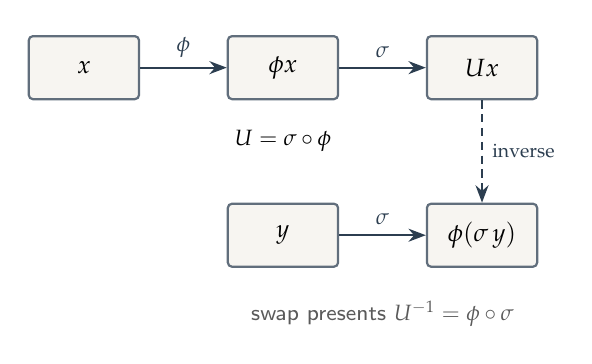
\begin{tikzpicture}[
  font=\small\sffamily,
  m/.style={draw=accent!75, fill=nodefill, thick, rounded corners=1.5pt,
    minimum width=14mm, minimum height=8mm, align=center},
  arr/.style={-{Stealth[length=2.2mm]}, accent, thick}
]
\node[m] (x) {$x$};
\node[m, right=11mm of x] (phix) {$\phi x$};
\node[m, right=11mm of phix] (ux) {$Ux$};
\draw[arr] (x) -- node[above, font=\footnotesize]{$\phi$} (phix);
\draw[arr] (phix) -- node[above, font=\footnotesize]{$\sigma$} (ux);
\node[m, below=13mm of ux] (rev) {$\phi(\sigma\,y)$};
\node[m, left=11mm of rev] (y) {$y$};
\draw[arr] (y) -- node[above, font=\footnotesize]{$\sigma$} (rev);
\draw[arr, densely dashed] (ux) -- node[right, font=\scriptsize]{inverse} (rev);
\node[below=2.5mm of phix, align=center, font=\footnotesize\sffamily]
  {$U=\sigma\comp\phi$};
\path (y.south) -- (rev.south)
  node[midway, below=3mm, align=center, font=\footnotesize\sffamily, text=muted]
    {swap presents $U^{-1}=\phi\comp\sigma$};
\end{tikzpicture}
\caption{Two-bounce presentation and swap. Pair labels are conventional;
exchange covers reversal (Theorem~\ref{thm:swap}).}
\label{fig:bounce}
\end{figure}

\begin{interpretation}
\label{int:mirrors}
In the dihedral picture~\cite{dihedral}, a rotation fixes the angle
between mirrors, not their absolute position. Theorem~\ref{thm:canonfail} is that fact on
finite carriers; Theorem~\ref{thm:swap} promotes the exchange.
\end{interpretation}


\section{Classification of couplings}
\label{sec:coupling}

\dep{Proposition~\ref{prop:no-erase} (in-arena losslessness);
Definition~\ref{def:twobounce}; Theorem~\ref{thm:canon} (pole gauge).}

The static classification earned the kernel by elimination. This
section earns the equation of motion the same way and is the twin of
Theorem~\ref{thm:ambient-unique} one level up. Fields take values in
the kernel carrier: a configuration is $u:\mathrm{Fin}\,n\to\Bool$, and
a state is the pair of the previous and the current configuration. The
candidate space is the general second-order nearest-neighbour update
\[
  u_{t+1}(i) \;=\; F\bigl(u_{t-1}(i),\,u_t(i{-}1),\,u_t(i),\,u_t(i{+}1)\bigr),
  \qquad F:\Bool^4\to\Bool,
\]
with $F$ arbitrary. Two stages eliminate every candidate except one
coupling up to pointwise flip.

\begin{theorem}[Losslessness selects the xor form]
\label{thm:toggle}
\textup{(i)}~If $F$ toggles in its previous-layer slot at every
neighbourhood, that is $F(\mathsf{true},l,m,r)\neq
F(\mathsf{false},l,m,r)$ for all $l,m,r$, then
\[
  F(p,l,m,r) \;=\; p \oplus G(l,m,r), \qquad
  G := F(\mathsf{false},\cdot,\cdot,\cdot).
\]
\textup{(ii)}~If $F$ fails to toggle at some neighbourhood, then two
histories on the three-ring agree after one step at every site while
differing at a site: the step erases, exhibited pointwise.
\end{theorem}

\begin{remark}[Status]
Proved. Clause~\textup{(i)} is \texttt{toggle\_forces\_xor\_form}
and clause~\textup{(ii)} is \texttt{collision\_of\_not\_toggling}
(bridge module \texttt{DynamicsAmbient}, (b); the first axiom-free,
the second \texttt{propext} only).
Losslessness therefore characterises the second-order xor structure:
the form is derived, and no separate choice of update shape enters.
Every xor-form step is lossless with an explicit two-bounce
factorisation, by the general theorems of
Section~\ref{sec:wave}.
\end{remark}

The residual freedom after Theorem~\ref{thm:toggle} is the coupling
$G:\Bool^3\to\Bool$. One restriction is declared rather than proved.

\begin{interpretation}[Inter-site restriction as signature]
\label{int:intersite}
The coupling is declared inter-site: it relates the two neighbours, and
the site's own influence is carried, exactly once, by the toggling
slot, leaving $K:\Bool\to\Bool\to\Bool$ with
$G(l,m,r)=K(l,r)$. This is a signature declaration in the exact style
of Interpretation~\ref{int:ambient}: it fixes the arity of the
interaction in daylight, just as Definition~\ref{def:arena} fixes one
type and one endomap. It is a declaration; no theorem is claimed for
it, and the status section records it beside the arena signature.
\end{interpretation}

\begin{theorem}[Coupling uniqueness]
\label{thm:coupling}
Let $K:\Bool\to\Bool\to\Bool$ satisfy
\begin{enumerate}[label=(\roman*)]
\item \textbf{parity}: $K(l,r)=K(r,l)$;
\item \textbf{pole invariance}: $K(\neg l,\neg r)=K(l,r)$;
\item \textbf{drawing condition}: $K$ takes two values.
\end{enumerate}
Then $K=\oplus$ pointwise or $K=\neg\comp\oplus$ pointwise.
\end{theorem}

\begin{remark}[Status]
Proved; \texttt{Bridge.DynamicsAmbient.coupling\_uniqueness}~(b),
axiom-free. The three ambient conditions mirror the static
classification. Parity bans a smuggled spatial arrow, as symmetric
step bans the smuggled temporal one. Pole invariance is respect for
the label gauge of Theorem~\ref{thm:canon}: a coupling that read the
absolute pole labels would export the content gauge of
Table~\ref{tab:gauges} into the dynamics. The drawing condition is
non-degeneracy: a coupling that draws no distinction couples nothing,
as a degenerate orbit carries no act. The two survivors form a single
orbit of the flip involution $K\mapsto\neg\comp K$
(\texttt{flip\_involution}, \texttt{survivors\_one\_orbit}, both (b)
and axiom-free); the gauge class of that flip is settled by a
carrier-size dichotomy in Section~\ref{sec:z2}.
\end{remark}

\begin{theorem}[The survivor is the wave coupling]
\label{thm:survivor}
Instantiated on the ring, the surviving coupling is the wave coupling
of Section~\ref{sec:wave} definitionally:
$c(i-1)\oplus c(i+1) = \mathrm{ringX}\,c\,i$ for every configuration
$c$ and site $i$.
\end{theorem}

\begin{remark}[Status]
Proved; \texttt{Bridge.DynamicsAmbient.survivor\_is\_wave\_coupling}~(b).
The proof term is \texttt{rfl}; the \texttt{propext} entry in its
footprint arrives through the $\mathrm{Fin}$ index arithmetic of the
neighbour offsets, which the statement itself mentions. The package
conjunction
\texttt{Bridge.DynamicsAmbient.dynamics\_ambient\_uniqueness}~(b),
\texttt{propext} only, assembles Theorems~\ref{thm:toggle},
\ref{thm:coupling}, and~\ref{thm:survivor}. The classified dynamics
therefore inherits, definitionally, the two-bounce form and the
swap-reversal of Section~\ref{sec:wave}.
\end{remark}

\begin{interpretation}
\label{int:twin}
The section is the dynamic twin of Theorem~\ref{thm:ambient-unique}.
There the one-variable equational ambient left $a\comp a=\mathrm{id}$
as the unique nontrivial equation banning smuggled arrow and smuggled
loss; here losslessness plus parity, pole invariance, and the drawing
condition leave one coupling up to flip. In both cases the surviving
object is forced by obstruction, the residual signature declaration is
made in daylight, and the residual two-element freedom is handed to
the gauge inventory of Section~\ref{sec:z2}.
\end{interpretation}


\section{Wave dynamics}
\label{sec:wave}

\dep{Theorem~\ref{thm:toggle}; Definition~\ref{def:twobounce};
Theorem~\ref{thm:swap}; ladder capacity for
Theorem~\ref{thm:recur}.}

The classified update is now developed as a dynamics. Over $\Bool$
with $\oplus$ as addition, the discrete d'Alembert form
$u_{t+1}=u_{t-1}+\Delta u_t$ becomes the second-order field equation
$\mathrm{step}\,X\,(s_1,s_2) = (s_2,\; i\mapsto s_1(i)\oplus X\,s_2\,i)$
on state pairs, with the spatial coupling $X$ kept general: every
theorem below holds for every coupling, and the classified survivor of
Section~\ref{sec:coupling} is one instance. Write
$\mathrm{swap}\,(s_1,s_2)=(s_2,s_1)$ for the channel swap and
$\mathrm{shear}\,X\,(s_1,s_2)=(i\mapsto s_1(i)\oplus X\,s_2\,i,\;s_2)$
for the coupling-controlled flip of the previous layer.

\begin{theorem}[The step is two bounces, definitionally]
\label{thm:wavebounce}
$\mathrm{step}\,X = \mathrm{swap}\comp\mathrm{shear}\,X$ holds by
definitional equality, and both factors are involutions. The
two-bounce factorisation of Definition~\ref{def:twobounce} holds here
by explicit construction, with the pair exhibited in closed form.
\end{theorem}

\begin{remark}[Status]
Proved; \texttt{Bridge.WaveDynamics.step\_eq\_two\_bounce}~(b),
axiom-free, with \texttt{swap\_involution} and
\texttt{shear\_involution\_pointwise} (both (b), axiom-free). Where
Theorem~\ref{thm:exists} extracts a factor pair by bounded search,
the wave step carries its pair on its face.
\end{remark}

\begin{theorem}[Reversal is the bounce swap]
\label{thm:wavereverse}
The reverse evolution $\mathrm{reverse}\,X :=
\mathrm{shear}\,X\comp\mathrm{swap}$ is presented by the swapped pair,
equals $\mathrm{swap}\comp\mathrm{step}\,X\comp\mathrm{swap}$
definitionally, and inverts the step on both layers in both
composition orders.
\end{theorem}

\begin{remark}[Status]
Proved; \texttt{reverse\_is\_swapped\_pair} and
\texttt{reverse\_step\_pointwise} (bridge module
\texttt{WaveDynamics}, both (b) and axiom-free) give the
pointwise cancellation; the packaged equality
\texttt{reverse\_step}~(b) lifts it to function level and carries
\texttt{Quot.sound} through an explicit \texttt{funext} step, made in
daylight. This instantiates Theorem~\ref{thm:swap} at field level:
channel swap covers time reversal for the classified dynamics.
\end{remark}

\begin{theorem}[Losslessness for every coupling]
\label{thm:wavelossless}
For every coupling $X$ and every carrier size, $\mathrm{step}\,X$ is
injective: no two histories merge.
\end{theorem}

\begin{remark}[Status]
Proved; \texttt{step\_lossless} (bridge module
\texttt{WaveDynamics}, (b)), inheriting the \texttt{Quot.sound}
(function extensionality) footprint of \texttt{reverse\_step}. The footprint split of this section is part of
the result and is preserved deliberately: the pointwise theorems and
Theorem~\ref{thm:wavebounce} are axiom-free, while the packaged
function-level equalities use \texttt{funext} by name, and the audit
flags exactly those uses (Section~\ref{sec:concl}).
\end{remark}

\begin{theorem}[Period spectrum: the gcd law]
\label{thm:gcd}
On $\mathrm{Fin}\,n$ the order of the $k$-th harmonic shift
$i\mapsto i+k$ is $n/\gcd(n,k)$: that count of beats returns every
point, and no smaller positive count fixes any point. Moreover every
injective endomap of a finite carrier is a composite of two
involutions, and every rotation is the composite of two explicit
arithmetic mirrors.
\end{theorem}

\begin{remark}[Status]
Proved; \texttt{order\_eq\_div\_gcd} (bridge module
\texttt{PeriodSpectrum}, (b); \texttt{propext} and
\texttt{Quot.sound} through library lemmas and \texttt{omega}, with
no function-extensionality step);
\texttt{overtone\_generation}~(b), axiom-free, via
Theorem~\ref{thm:exists}; \texttt{rot\_eq\_two\_flips} and the
packaged computable witness \texttt{rotFactor} (both (b),
\texttt{propext} and \texttt{Quot.sound}). On a finite carrier the
honest surrogate for frequency is order, and order ratios stand in
for frequency ratios; real frequencies are refused
(Section~\ref{sec:status}).
\end{remark}

The twelve-carrier is the worked instance of the law: interval
composition adds shifts
(\texttt{interval\_addition}~(b), axiom-free), every harmonic is an
iterate of the fundamental step
(\texttt{harmonics\_are\_iterates}~(b), \texttt{propext}), the whole
tone has order six, the major third order three, and the tritone
order two (\texttt{orders\_twelve}~(b), \texttt{propext}), and the
circle of fifths closes after twelve steps and at no positive step
before (\texttt{circle\_of\_fifths}~(b), \texttt{propext} and
\texttt{Quot.sound}), each a decidable instance of
Theorem~\ref{thm:gcd}. The musical names are decoration and carry no
acoustic claim.

\begin{theorem}[Boundary conditions select the spectrum]
\label{thm:spectrumbc}
With the same rule and the same single-pulse initial state on four
sites, the periodic ring returns with state period $4$ and the
fixed-end line returns with state period $10$, each period exact.
\end{theorem}

\begin{remark}[Status]
Proved by kernel decision;
\texttt{Bridge.WaveDynamics.ring4\_period\_four} and
\texttt{dirichlet4\_period\_ten} (both (b), \texttt{propext} and
\texttt{Quot.sound} through the \texttt{Decidable} instances).
Boundary alone reshapes the spectrum. The closed-form period law in
general $n$ is refused pending the $\mathbb{F}_2[x]/(x^n-1)$
transfer-matrix algebra (Section~\ref{sec:status}); the annex retains
the kernel-decided period table at further small sizes.
\end{remark}

\begin{theorem}[Recurrence within capacity]
\label{thm:recur}
For every coupling $X$ and every state $s$ on $n$ sites there is a
positive $p\le 2^n\cdot 2^n = 2^{2n}$ with
$\mathrm{step}\,X^{\,p}(s)=s$ pointwise on both layers: losslessness
plus finite capacity forces exact return within the state-space
capacity of the carrier.
\end{theorem}

\begin{remark}[Status]
Proved; \texttt{Bridge.Recurrence.wave\_recurrence\_bounded}~(b),
\texttt{propext} and \texttt{Quot.sound}, with
\texttt{wave\_recurrence} and \texttt{wave\_recurrence\_pow}
inheriting the footprint. The pigeonhole is constructive: a bounded
decidable search replaces classical witness extraction, and
\texttt{Classical.choice} is absent from the footprint and from the
package. One \texttt{funext} step packages the colliding states
before cancellation; the step is essential for the general statement,
since the coupling is an arbitrary functional on fields, and the audit
flags it by name. Capacity language only: no ledger claim is made
here.
\end{remark}


\section{Archive and capacity}
\label{sec:archive}

\dep{ladder carrier (Section~\ref{sec:ladder}) as environment;
registration (Theorem~\ref{thm:reg}).}

\begin{theorem}[Archive and capacity]
\label{thm:caps}
Taking the environment at horizon $T$ to be the ladder carrier at
level~$T$, the committed capacity schedule satisfies
$|\mathrm{caps}\,T|=2^{T+2}$. Joint injectivity, merge, muting, and
confinement imply the combinatorial bound $K^{T}\le|\mathrm{caps}\,T|$;
at $K=2$ the committed ladder is eternally alive by arithmetic.
\end{theorem}

\begin{remark}[Status]
Proved in the dynamics layer. Continuum area or continuum entropy
identifications are refused.
\end{remark}


\section{Arrow as address}
\label{sec:arrow}

\dep{registration and archive growth.}

\begin{theorem}[Arrow reading]
\label{thm:arrow}
The dynamical arrow---archive ascent under registration---is identified
with address valued in $\{\mathsf{fwd},\mathsf{rev}\}$. Tick identification
(naming tick with microtick) holds for the classified fragment of
uniform free archives up to record gauge; periodic fund-exempt dynamics
and swap necessity are part of that classification.
\end{theorem}

\begin{remark}[Status]
Proved as a classified package in the dynamics layer. Record gauge is
packaging: exported only inside ``up to record gauge'' clauses.
\end{remark}

\begin{remark}[Return and ascent]
\label{rem:returnascent}
Theorem~\ref{thm:recur} sharpens the arrow reading. Within a level the
classified dynamics is recurrent: every state returns within capacity,
so no orbit inside a fixed carrier distinguishes a direction. Across
levels the ladder ascends and never retracts
(Theorem~\ref{thm:ladder}). Within a level time is return, across
levels time is ascent, and duration carries the direction: the arrow
of Theorem~\ref{thm:arrow} is the address on ascent, and the
recurrence bound says exactly why no substitute arrow is available
inside a level.
\end{remark}


\Needspace{18em}
\section{One underdetermination and gauges}
\label{sec:z2}

\dep{pole swap from Theorem~\ref{thm:canon}; address from
Theorem~\ref{thm:arrow}; channel from Definition~\ref{def:twobounce} and
Theorem~\ref{thm:swap}; coupling flip from Theorem~\ref{thm:coupling}.}

\begin{theorem}[One $\Ztwo$, three faces]
\label{thm:z2}
There is a single two-element underdetermination with three named
involutive projections:
\begin{center}
pole swap \quad$\cong$\quad
address $\{\mathsf{fwd},\mathsf{rev}\}$ \quad$\cong$\quad
channel $\{\varphi,\sigma\}$.
\end{center}
Each projection is an involution on a common $\Ztwo$ carrier.
\end{theorem}

\begin{figure}[ht]
\centering
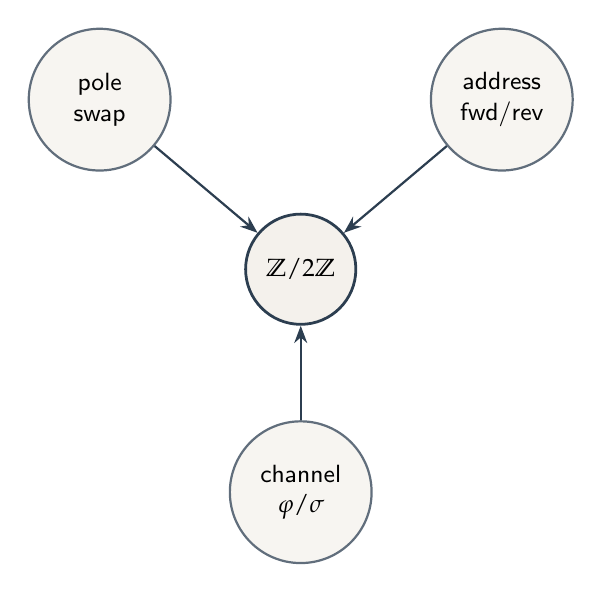
\begin{tikzpicture}[
  font=\small\sffamily,
  face/.style={draw=accent!75, fill=nodefill, thick, circle,
    minimum size=18mm, align=center, inner sep=1pt},
  hub/.style={draw=accent, fill=soft, thick, circle,
    minimum size=14mm, align=center, line width=1pt}
]
\node[hub] (z) {$\Ztwo$};
\node[face, above left=10mm and 14mm of z] (p) {pole\\swap};
\node[face, above right=10mm and 14mm of z] (a) {address\\fwd/rev};
\node[face, below=12mm of z] (c) {channel\\$\varphi/\sigma$};
\draw[-{Stealth[length=2.2mm]}, accent, thick] (p) -- (z);
\draw[-{Stealth[length=2.2mm]}, accent, thick] (a) -- (z);
\draw[-{Stealth[length=2.2mm]}, accent, thick] (c) -- (z);
\end{tikzpicture}
\caption{Three faces of one underdetermination (Theorem~\ref{thm:z2}).
Faces are presentations; the group is stated once.}
\label{fig:z2}
\end{figure}

\begin{definition}[Content vs packaging]
\label{def:gauge}
A gauge is \emph{content} when some exported statement mentions the
choice. A gauge is \emph{packaging} when the choice is quotiented before
downstream consumption.
\end{definition}

\begin{definition}[Kernel admission interface]
\label{def:admit}
A \emph{Bool kernel certificate} is a structure on kernel exports
(symmetry endomap, observation map, fixed locus) satisfying the
admission clauses: square of the symmetry is an involution; observation
intertwines the symmetry with negation; the fixed locus matches the
symmetry's fixed points and is classified empty or nonempty; and the
no-solo-cross no-go holds. Admission is a predicate on that interface.
\end{definition}

\begin{center}
\captionof{table}{Gauge demarcation protecting the single dictionary $\Ztwo$.}
\label{tab:gauges}
{\small
\begin{tabular}{@{}lll@{}}
\toprule
Gauge & Locus & Class \\
\midrule
Label / pole swap & Theorem~\ref{thm:canon} & content \\
Address fwd/rev & Theorem~\ref{thm:arrow} & content \\
Channel swap & Theorem~\ref{thm:swap} & content \\
Face representative (equivariant certs)
  & Theorem~\ref{thm:face-eq} & packaging \\
Record gauge per tick & Theorem~\ref{thm:arrow} & packaging \\
Factorisation gauge per step & Theorems~\ref{thm:exists}--\ref{thm:canonfail}
  & packaging \\
Coupling flip & Theorem~\ref{thm:flipgauge} & packaging iff $4\mid n$; else content \\
\bottomrule
\end{tabular}}
\end{center}

\begin{theorem}[Face-swap equivariance]
\label{thm:face-eq}
Admission for a Bool kernel certificate
(Definition~\ref{def:admit}) is stable under the $\Ztwo$ face/pole swap:
any admitted certificate remains admitted after conjugation by the face
involution. Consequently, for equivariant consumers of the admission
interface, choice of face is packaging in the sense of
Definition~\ref{def:gauge} and belongs in Table~\ref{tab:gauges}.
\end{theorem}

\begin{remark}[Status]
Theorem~\ref{thm:z2}, Definition~\ref{def:gauge}, and
Theorem~\ref{thm:face-eq} keep one dictionary $\Ztwo$: factorisation
non-uniqueness (Theorem~\ref{thm:canonfail}) is packaging; channel
\emph{labels} are conventional; channel \emph{swap} is content. Gauge
class is relative to locus
(Definition~\ref{def:gauge}): the same $\Ztwo$ choice may be content at
the kernel-export locus---exported statements mention it in ``up to
label swap'' clauses---and packaging at the certificate-consumption
locus, where equivariance lets the consumer quotient it. Pole / face
choice is the worked example of that locus-relative demarcation. If a
certificate breaks equivariance by fixing an orientation, that
orientation is certificate-supplied data and is audited there; kernel
exports remain swap-equivariant either way. The content/packaging
demarcation is a formal analogue of the question which symmetries carry
representational significance~\cite{bradingcastellani,dewar};
underdetermination by label swap is the formal shadow of
permutation-style underdetermination of reference~\cite{quine,putnam}.
\end{remark}

\paragraph{The coupling flip.}
The dynamic classification hands the inventory one further
involution. The two surviving couplings of Theorem~\ref{thm:coupling}
form a single orbit of the flip $K\mapsto\neg\comp K$ on coupling
space (\texttt{survivors\_one\_orbit}~(b), axiom-free). Pole
conjugation fixes each survivor, since pole invariance is a
hypothesis of the classification, so the flip is an involution
distinct from the pole face, and its class under
Definition~\ref{def:gauge} requires a proof before the inventory can
claim completeness. The following theorem supplies the proof, and the
answer depends on the carrier size.

\begin{theorem}[Coupling-flip dichotomy]
\label{thm:flipgauge}
On the ring with $n$ sites, write $\mathrm{step}$ for the dynamics of
the surviving coupling $\oplus$ and $\overline{\mathrm{step}}$ for
the dynamics of its flip $\neg\comp\oplus$.
\begin{enumerate}[label=(\roman*)]
\item If $4\mid n$, the two dynamics are conjugate by an explicit
involution of the state space: masking both layers by the
half-period pole mask $i\mapsto (2\le i \bmod 4)$ intertwines
$\mathrm{step}$ with $\overline{\mathrm{step}}$ exactly.
\item If $4\nmid n$, no map of state spaces intertwines the two
dynamics, injective or otherwise; in particular no state-space
bijection conjugates them. The obstruction is observable:
$\mathrm{step}$ fixes the zero state definitionally, while
$\overline{\mathrm{step}}$ fixes no state at all, because the
current layer of a fixed state would be an alternating mask, and
alternating masks exist exactly when $4\mid n$.
\item At every $n$ and every time $T$, the flipped evolution equals
the plain evolution dressed by a pair of constant pole masks drawn
from a period-four tick schedule (identity; flip the current layer;
flip both layers; flip the previous layer).
\end{enumerate}
\end{theorem}

\begin{remark}[Status]
Proved. The declarations reside in the quarantined experimental
package and are flagged as such, in the manner of
Section~\ref{sec:boundary}:
\texttt{Experimental.CouplingGauge.coupling\_flip\_dichotomy}~(e)
packages clauses (i) and (ii) from
\texttt{flip\_conjugacy\_of\_four\_dvd} and
\texttt{flip\_no\_intertwiner}; clause (iii) is
\texttt{flip\_iter\_dress\_pointwise}; the mask existence law is
\texttt{alternating\_mask\_iff\_four\_dvd} (all (e)). Footprints stay
within \texttt{propext} and \texttt{Quot.sound}: the dichotomy and
its conjugacy direction carry one direct \texttt{funext} step,
packaging the pointwise conjugacy in
\texttt{flip\_conjugacy\_of\_four\_dvd}, flagged by name in the
audit, and the remaining entries arrive through the $\mathrm{Fin}$
index arithmetic of the coupling, \texttt{omega}, and kernel-decided
\texttt{Decidable} instances. Concrete exhibits
instantiate the dichotomy: single-pulse state periods under the
flipped coupling at sizes $2$, $3$, $5$ are $4$, $12$, $20$ against
the plain $2$, $6$, $10$, and size $4$ keeps its period $4$, as the
conjugacy requires (\texttt{flip\_ring2\_pulse\_period\_four} through
\texttt{flip\_ring5\_pulse\_period\_twenty}, all (e); the first three
are kernel-decided, and the five-site exhibit is assembled through
the dressing, with kernel decisions confined to the ten plain
states of its period).
\end{remark}

The flip is thereby placed, and Table~\ref{tab:gauges} records the
row with its dichotomy. On carriers divisible by four the flip is
packaging in the sense of Definition~\ref{def:gauge}: the conjugating
mask lets any consumer of the dynamics quotient the choice of
representative before consumption. On every other carrier the two
dynamics are observably distinct and admit no equivariant
identification, so there the flip carries content, and the surviving
pair is exported only inside ``up to coupling flip'' clauses,
mirroring the label-swap treatment. Clause (iii) explains the near
miss with the record gauge of Theorem~\ref{thm:arrow}: the flip is a
per-tick repackaging at every size, and outside the divisible sizes
the tick schedule can be traded for no single time-independent map.
The single dictionary $\Ztwo$ of Theorem~\ref{thm:z2} is unaffected
at every size, because the classification is exported only as the
orbit $\{\oplus,\neg\comp\oplus\}$, every theorem of
Section~\ref{sec:wave} holds for every coupling, and no downstream
consumer selects a representative, so the flip never reaches the
dictionary layer and the count of dictionary underdeterminations
remains one. With the row decided, the completeness claim for the
inventory carries no proviso.


\section{The boundary}
\label{sec:boundary}

\dep{Theorem~\ref{thm:seal} (seal); Definition~\ref{def:ladder} and
Theorem~\ref{thm:ladder} (ladder); Theorem~\ref{thm:canon} (pole
swap).}

The ladder ascends without end; this section examines its edge. A
\emph{complete gauge history} is one pole choice at every level
forever, an element of $\mathbb{N}\to\Bool$; the space of complete
gauge histories is the \emph{boundary}. No cardinality claim beyond
the seal is made or needed. The declarations of this section reside in
the quarantined experimental package (package letter e); every one of
them is axiom-free, and the audit records them per declaration.

\begin{theorem}[Rungs embed with effective separation]
\label{thm:rungs}
Every ladder level embeds injectively in the boundary, and the
injectivity is effective: distinct inhabitants of level $k$ differ at
some coordinate $m\le k$ of their encodings, so depth-$(k{+}1)$
cylinders separate level $k$. The fundamental embeds as the two
constant histories, and the ladder's climb-then-drop step is carried
at the boundary by prepend and tail as a section/retraction pair.
\end{theorem}

\begin{remark}[Status]
Proved; \texttt{rungs\_embed}, \texttt{encode\_separates},
\texttt{fundamental\_embeds}, and \texttt{tail\_encode\_some}
(experimental module \texttt{CantorBoundary}, all (e) and
axiom-free). The separation
bound is explicit, so the embedding is a finite-approximation
statement and no choice principle enters.
\end{remark}

\begin{theorem}[The boundary seals at its own carrier]
\label{thm:boundaryseal}
The pole swap lifts to the boundary as the coordinatewise flip, the
lift is a pointwise involution, and it is live: it moves every
history. Consequently no map $f:A\to A\to(\mathbb{N}\to\Bool)$ is
point-surjective, for any carrier $A$: the boundary is itself a live
arena, sealed at its own carrier by its own act.
\end{theorem}

\begin{remark}[Status]
Proved; \texttt{flip\_live} and \texttt{boundary\_seals\_itself}
(experimental module \texttt{CantorBoundary}, both (e) and
axiom-free). This
strengthens the observation that no enumeration reaches the boundary
(\texttt{boundary\_unenumerable}, the corpus seal specialised to
carrier $\mathbb{N}$): here the sealing act lives on the boundary
itself. The one $\Ztwo$ also acts at infinite depth: masking by a
history is a pointwise involution, and the mask at the all-true
history is the lifted pole swap.
\end{remark}

\begin{theorem}[The tail step erases]
\label{thm:tailerase}
The tail step on histories, dropping the first pole choice, is
erasing: the constantly-false history and the history that spikes only
at coordinate $0$ differ, and their tails are definitionally equal.
The tail nevertheless has a section per pole choice: prepending either
pole and then taking the tail restores every coordinate.
\end{theorem}

\begin{remark}[Status]
Proved; \texttt{tail\_erasing} and \texttt{tail\_cons}
(experimental module \texttt{CantorBoundary}, both (e) and
axiom-free; the erasure witness is definitional). The reframed law reads: \emph{losslessness is a
finite-stage theorem, and its failure at the colimit is itself a
theorem.} In the arena, involutivity excludes erasure
(Proposition~\ref{prop:no-erase}); at every finite carrier the
classified dynamics is injective for every coupling
(Theorem~\ref{thm:wavelossless}); at the boundary the tail step
erases. The loss is recorded as the system's one structural loss, a
poverty of the edge stated with the same prominence as the finite-stage
exclusions, and Section~\ref{sec:status} carries it in the residue
accounting.
\end{remark}

\begin{interpretation}
\label{int:boundary}
The completion has the form of the system. The boundary carries a
live symmetric act (the lifted pole swap), and it is self-opaque in
the same sense as every level (Theorem~\ref{thm:boundaryseal}), so
the colimit does not step outside the shape it completes. At the same
time the excluded shape returns at infinity: erasure, priced out of
the arena at every finite stage, reappears as the tail step of the
completed object. The edge of the system is systematic in form and
lossy in dynamics, and both halves are theorems.
\end{interpretation}


\section{Self-articulation}
\label{sec:selfart}

\dep{Theorem~\ref{thm:canon} (initiality); Theorems~\ref{thm:seal},
\ref{thm:ladder}, \ref{thm:corpus}; Theorem~\ref{thm:z2} (pole gauge).}

The classification ends in one survivor; this section states what the
survivor's self-relation supports. Three candidate readings are on the
table: (a)~world is the structured self-articulation of the canon, with
questions of witness and standpoint arising only inside the descriptive
field that articulation generates; (b)~given the kernel, worldhood
\emph{necessarily} arises as self-presentation; (c)~reality \emph{is}
the self-appearance of the involutive survivor. The theorems below
support a conditional form of~(a); readings (b) and~(c) are refused
(Section~\ref{sec:status}).

\begin{definition}[Presentation]
\label{def:pres}
Let $\act:\beta\to\beta$ and $z:\beta$. A \emph{presentation} of the
canon at the standpoint $(\beta,\act,z)$ is a map $g:\beta\to\Bool$ with
$g(z)=\mathrm{true}$ and $g(\act\,x)=\neg g(x)$ for all $x$.
\end{definition}

\begin{theorem}[No second term]
\label{thm:noext}
\textup{(A)}~For every carrier $W$ and every self-reading
$r:W\to W\to\Bool$, $r$ is sealed and fails to articulate its own
dodge; witnessing confers no exemption from the interior triad.
\textup{(B)}~Every presentation forces liveness of its standpoint
everywhere, retracts the canon's articulation
($g\comp\mathrm{reading}=\mathrm{id}$ on $\Bool$), and renders the
articulation into the standpoint injective, so the standpoint contains
the canon. \textup{(C)}~On a generated carrier the presentation is
unique.
\end{theorem}

\begin{remark}[Status]
Proved; every clause of Theorem~\ref{thm:noext} is axiom-free
(declaration \texttt{no\_exterior\_standpoint}, spine module
\texttt{NoExterior}). The retraction clause is
the exact content of reading~(a): a second term's view of the canon is
the canon's self-articulation read back, and clause~\textup{(C)} leaves
the view no independent content.
\end{remark}

\begin{theorem}[Witness lands in the pole gauge]
\label{thm:preswit}
A context-free live witness ($\mathrm{TDiff}$ together with
$\mathrm{Alive}$ at the seed) determines a presentation up to pole
swap: some presentation agrees with the witness or with its pointwise
flip. The residual choice is the label gauge of Table~\ref{tab:gauges}
and nothing else.
\end{theorem}

\begin{theorem}[Retorsion]
\label{thm:retorsion}
Write $\mathrm{Draws}\,M$ for the existence of two distinct elements of
$M$. If a map $t:\mathrm{Prop}\to M$ assigns distinct values to
$\mathrm{Draws}\,M$ and to its negation, then $\mathrm{Draws}\,M$
holds.
\end{theorem}

\begin{remark}[Status]
Proved (\texttt{Monism.retorsion}); the two registered values
themselves witness the distinction. The theorem draws the codomain:
what a registered denial establishes is that the medium of registration
is already distinguished. Section~\ref{sec:status} relocates the
existential residue accordingly.
\end{remark}

\begin{theorem}[Self-articulation]
\label{thm:selfart}
The following conjunction holds. \textup{(I)}~Retorsion, as in
Theorem~\ref{thm:retorsion}. \textup{(II)}~On any carrier with a drawn
distinction, a symmetric generated act is live and involutive and reads
as negation from every seed, exhaustively and injectively.
\textup{(III)}~Every ladder level self-represents under seal,
self-opacity, and outrun. \textup{(IV)}~No exterior standpoint, as in
Theorem~\ref{thm:noext}. \textup{(V)}~Names lag predicates at every
level, the lag recedes under completion, and the $\omega$-colimit
embeds in no level (every level, meanwhile, embeds effectively in the
boundary of Section~\ref{sec:boundary}, which is sealed at its own
carrier and erases at its tail).
\end{theorem}

\begin{remark}[Status]
Proved as a single declaration (\texttt{self\_articulation}, spine
module \texttt{SelfArticulation}; footprint \texttt{propext} only). The antecedent of clause~\textup{(II)} is the
drawn distinction \emph{together with} the ambient equations, whose
adequacy within the one-variable fragment is
Theorem~\ref{thm:ambient-unique}; the package does not derive the
ambient from $\mathrm{Draws}$ alone. The parenthetical in
clause~\textup{(V)} is a cross-reference: the non-injection is part of
the packaged declaration, while the boundary facts it points to are
Theorems~\ref{thm:rungs}--\ref{thm:tailerase} at their own package.
\end{remark}

\begin{interpretation}
\label{int:selfart}
Reading~(a) is adopted in conditional form. Given one drawn
distinction, articulation as negation is forced~\textup{(II)},
standpoints arise as inhabitants of the articulation~\textup{(III)},
any presentation to a second term returns the articulation
itself~\textup{(IV)}, and the whole exists only as
duration~\textup{(V)}. Questions of witness, standpoint, and medium are
well-posed from level~1 upward because the vocabulary that poses them
is generated by the ascent. ``World'' names the consequent of this
conditional; the identification is interpretation, and the sentence
that the only complete description of the system is the system is a
gloss on the non-injection of clause~\textup{(V)}. The consequent's
dynamics is itself classified: given the antecedent, the kernel is
forced (Theorem~\ref{thm:canon}) and its equation of motion is forced
up to the coupling flip (Section~\ref{sec:coupling}), whose own gauge
class is decided by Theorem~\ref{thm:flipgauge}, so the conditional
package carries both its kinematics and its dynamics. Readings (b)
and~(c) are refused: (b)~asserts necessity while the corpus carries no
modal apparatus, and (c)~discharges the existential residue while
Section~\ref{sec:status} declines that discharge. Retorsion narrows
what the refusal of~(c) costs: any registered denial of the antecedent
draws its own medium, so the undischarged step runs from registered
distinction to world, and only that step.
\end{interpretation}


\section{Dictionary: two certificates}
\label{sec:dict}

\dep{Definition~\ref{def:admit}; Theorem~\ref{thm:selfart};
Sections~\ref{sec:coupling}--\ref{sec:wave} for the second exhibit.}

The dictionary layer admits physical or contemplative identifications
by certificate only. This paper works two exhibits. The first is
contemplative, chosen because its subject matter coincides with the
corpus's own: reflexive self-representation. The second is physical
and identifies the classified dynamics with reversible lattice
computation.

\begin{interpretation}[Meta-problem certificate]
\label{int:dict}
Chalmers's meta-problem asks why physical systems \emph{report} an
explanatory gap~\cite{chalmers}. The certificate instantiates
Definition~\ref{def:admit} at the self-ascription bit: the symmetry is
the live flip, observation is the identity reading, and the fixed locus
is classified empty, so awareness in this model is always awareness of
a distinction. Admission holds
(\texttt{Dictionary.MetaProblem.meta\_admitted}), and the report
skeleton is theorem-shaped at every ladder level: self-opacity (the
dodge is never articulated), outdated portrait (each completed
self-model is outrun), and restless signature (no tracked
self-ascription stabilises), each at the quantitative grade of
Theorem~\ref{thm:corpus}. Systems satisfying these clauses report
ineffability and incompleteness on structural grounds.
\end{interpretation}

\begin{remark}[Status]
Layer~3 only; no theorem of Sections~\ref{sec:class}--\ref{sec:selfart}
depends on it. The hard problem is untouched by design: nothing here
says why there is something it is like to be such a system, and qualia
claims are refused (Section~\ref{sec:status}).
\end{remark}

\begin{interpretation}[Reversible-computation certificate]
\label{int:dict2}
The classified dynamics of
Sections~\ref{sec:coupling}--\ref{sec:wave} is a reversible lattice
dynamics in the mathematical sense: a second-order update on a finite
carrier, injective for every coupling
(Theorem~\ref{thm:wavelossless}), factored into two involutions with
reversal by their exchange (Theorems~\ref{thm:wavebounce}
and~\ref{thm:wavereverse}), and recurrent within capacity
(Theorem~\ref{thm:recur}). The certificate identifies this object
with reversible lattice computation in the tradition of Fredkin and
Toffoli~\cite{fredkintoffoli} and of invertible cellular
automata~\cite{toffolimargolus,margolus}: sites are cells, the
microstep is an invertible update, losslessness is logical
reversibility in Bennett's sense~\cite{bennett}, and the two-bounce
presentation is the decomposition of an invertible dynamics into
involutions familiar from that literature and from reversing
symmetries~\cite{lambroberts}. The identification is admitted through
the interface of Definition~\ref{def:admit}: the symmetry endomap is
the live flip the dynamics toggles, observation is the identity
reading, the fixed locus is classified empty, and the admission
clauses hold on those exports. The exhibit is earned in a way the
Landauer reading of registration~\cite{landauer} alone was not: the
object on the corpus side is now classified rather than posited, so
the certificate attaches physics to a forced structure.
\end{interpretation}

\begin{remark}[Status]
Layer~3 only, as always: the identification is confined to this
certificate, no theorem of
Sections~\ref{sec:class}--\ref{sec:selfart} depends on it, and the
words ``computation'' and ``cell'' import nothing upward. Physical
certificates (registration as dissipation in the sense of
Landauer~\cite{landauer}, with further exhibits retained in the
corpus) instantiate the same admission interface; that shared
interface is the only correspondence between physical and
contemplative readings asserted here.
\end{remark}


\section{Open, refused, and philosophical}
\label{sec:status}

\begin{statusopen}
Continuum Lorentzian structure and boosts (no continuous
one-parameter subgroup from a single $\Ztwo$); sheaf assembly beyond
combinatorial stalk agreement; recombination budget versus
ultrametric obstruction; alphabet-lift beyond the Fin interfaces
closed here.
\end{statusopen}

\begin{statusrefused}
Premise-free global laws of time; continuum Einstein equations as
theorems of this corpus; host-logic incompleteness; G\"odel
arithmetisation of the formal text; experiential or qualia claims;
derivation of the world from $\Bool$ alone (including any discharge of
the existential residue below); modal strengthening of the
self-articulation package of Theorem~\ref{thm:selfart} (the corpus
carries no modal apparatus); ambients beyond the one-variable
equational fragment of the arena signature (including multi-variable
single equations treated as ambients, quasi-equational, and Horn /
second-order constraints), refused by parsimony of the arena language;
the closed-form period law of the classified dynamics in general $n$,
pending the $\mathbb{F}_2[x]/(x^n{-}1)$ transfer-matrix algebra absent
from a Lean-core-only corpus; dispersion relations; continuum
frequencies (on a finite carrier, order is the honest surrogate, per
Theorem~\ref{thm:gcd}).
\end{statusrefused}

\begin{statusphil}
Residue accounting, with the prior items replaced by theorem citations.
\begin{enumerate}[label=(\roman*)]
\item \textbf{Registration residue.} A registration occurs. Retorsion
(Theorem~\ref{thm:retorsion}) converts any assignment that registers
the denial of a drawn distinction distinctly from its affirmation into
a proof that the registering carrier is drawn, and orbit liveness is
Theorem~\ref{thm:live-orbit}; the residue is thereby relocated from the
existence of a non-degenerate act to the occurrence of one
registration. The corpus exhibits a two-point model witnessing the
existential and declares no axiom, so the residue is carried as an
architectural note in the audit: what remains undischarged is the
interpretive step from registered distinction to world, and that
discharge is refused.
\item \textbf{Signature declaration.} Arena data as given
(Definition~\ref{def:arena}: one type, one endomap). Adequacy of
$a\comp a=\mathrm{id}$ is Theorem~\ref{thm:ambient-unique}; the signature
choice is opening definition, not residue.
\item \textbf{Equivariance discipline.} Face choice under the kernel
admission interface (Definition~\ref{def:admit}) is packaging or
certificate-supplied data
(Theorem~\ref{thm:face-eq}; Table~\ref{tab:gauges}).
\item \textbf{Erasure at the edge.} Losslessness is a finite-stage
law: the arena excludes erasure by involutivity
(Proposition~\ref{prop:no-erase}), and the classified dynamics is
injective for every coupling at every finite carrier
(Theorem~\ref{thm:wavelossless}). At the colimit the exclusion fails,
and the failure is itself a theorem
(Theorem~\ref{thm:tailerase}): the tail step on complete gauge
histories erases. The residue here is a reclassification of the
corpus's self-description, carried as the system's one structural
loss; it is recorded, and no repair is attempted.
\item \textbf{Coupling signature.} The inter-site arity of the
coupling (Interpretation~\ref{int:intersite}) is a signature
declaration beside the arena signature of item~(ii); adequacy of the
three ambient conditions given that signature is
Theorem~\ref{thm:coupling}.
\end{enumerate}
\noindent
The pattern across all five is the same: each item of residue is
reclassified, whether as a theorem over an exhaustively specified search
space, as an audited residue at the base, or as certificate-supplied
data. The irreducible core is the
existence of one distinction: the sole existential residue and the sole
dictionary underdetermination are the same $\Ztwo$; the coupling flip
is placed by Theorem~\ref{thm:flipgauge} and stays out of the
dictionary count, because every downstream consumer receives the
dynamics coupling-uniformly.
\end{statusphil}


\section{Relation to prior work}
\label{sec:related}

\paragraph{Diagonal and fixed-point arguments.}
The seal (Theorem~\ref{thm:seal}) instantiates Lawvere's diagonal
schema~\cite{lawvere}, the common form of Cantor's
theorem~\cite{cantor} and, via arithmetisation, of G\"odel's first
incompleteness theorem~\cite{godel}; Yanofsky~\cite{yanofsky} surveys
the family. Those applications fix a logical or set-theoretic universe
and derive a limitative theorem inside it. Here the carrier of the
diagonal argument is itself the output of the classification
(Sections~\ref{sec:class}--\ref{sec:fund}): the seal is a structural
property of any fundamental act, not of a formal system. No
arithmetisation is performed, and host-logic incompleteness is refused,
not claimed (Section~\ref{sec:status}).

\paragraph{Reversible computation and reversible cellular automata.}
Reading injectivity as ``no erasure'' follows the logical-reversibility
tradition~\cite{bennett,fredkintoffoli}, with Landauer's
principle~\cite{landauer} as its thermodynamic counterpart. That
literature takes reversibility as a premise about computing machinery.
Here losslessness is not a premise: erasure is excluded in-arena by one
equation (Proposition~\ref{prop:no-erase}), and reversibility of
forward microsteps is recovered by the two-bounce factorisation
(Theorems~\ref{thm:converse}--\ref{thm:exists}). The classified wave
dynamics of Section~\ref{sec:wave} additionally places the corpus
beside the invertible cellular automata and lattice dynamics
literature~\cite{toffolimargolus,margolus,kari}: second-order
(memory) constructions are a standard route to invertible lattice
rules there, and the $\mathrm{step}/\mathrm{swap}/\mathrm{shear}$
presentation is of that family. The direction of derivation differs
in the same way: that literature engineers invertible rules and
studies their power, while here the second-order form and the
coupling are outputs of an eliminative classification
(Section~\ref{sec:coupling}). The thermodynamic and computational
readings survive only as dictionary certificates
(Section~\ref{sec:dict}).

\paragraph{Uniqueness of update rules.}
The coupling classification (Theorem~\ref{thm:coupling}) is a
uniqueness result for a cellular-automaton-style rule: constraints on
the local rule (injectivity of the global map, symmetry of the
neighbourhood action, invariance under the alphabet involution,
non-degeneracy) pin the rule down to a two-element orbit. The
cellular automata literature studies the corresponding decision
problems and structure theory: injectivity and surjectivity of the
global map from the local rule~\cite{amorosopatt}, and the general
theory of reversible automata~\cite{kari,toffolimargolus}. Those
results characterise which rules have a property across a rule space;
the result here runs the other way and asks which rules survive a
conjunction of ambient demands, with the answer being a single orbit.
The residual flip is placed by proof: packaging exactly on carriers
divisible by four, content elsewhere (Section~\ref{sec:z2}).

\paragraph{Involutions and reversing symmetries.}
That every finite permutation is a product of two involutions is
classical~\cite{petersentenner}, as is the dihedral factorisation of a
rotation into reflections~\cite{dihedral}; maps so factorised are the
reversible maps of dynamical-systems theory~\cite{lambroberts}. The
contribution here is not the existence of the factorisation but the
disposition of its non-uniqueness: canonicity fails
(Theorem~\ref{thm:canonfail}), the failure is classified as packaging
rather than content (Definition~\ref{def:gauge}), and channel
swap---which is content---covers step reversal independently of the
chosen factorisation (Theorem~\ref{thm:swap}).

\paragraph{Symmetry and underdetermination.}
Which symmetries carry representational significance is a standing
question in the philosophy of physics~\cite{bradingcastellani,dewar};
permutation-style underdetermination of reference descends from
Quine~\cite{quine} and Putnam's model-theoretic argument~\cite{putnam}.
Those debates are conducted informally over rich physical or semantic
theories. The analogue here is deliberately narrow: the
content/packaging distinction is a definition in the formal text
(Definition~\ref{def:gauge}), each gauge is classified by theorem
(Table~\ref{tab:gauges}), and the residual underdetermination is
exactly inventoried---one $\Ztwo$, three faces (Theorem~\ref{thm:z2}).
Nothing is asserted about physical theories; within its scope the
inventory is machine-checked, and its last row to be placed, the
coupling flip, is decided by the carrier-size dichotomy of
Section~\ref{sec:z2}.

\paragraph{Self-articulation and the mark.}
The nearest formal ancestor of the self-articulation package is
Spencer-Brown's calculus of the first distinction~\cite{spencerbrown},
with Varela's extension for re-entry~\cite{varela}; the classical
antecedents are Fichte's self-positing act~\cite{fichte} and Hegel's
self-relating negativity~\cite{hegel}. Those systems posit the
reflexive structure as primitive or develop it inside an informal
dialectic. Here the two-cycle is the survivor of an eliminative
classification, re-entry is replaced by a ladder whose ascent is a
theorem, the residual underdetermination is inventoried as one
$\Ztwo$, and the single undischarged bit is audited
(Section~\ref{sec:status}).

\paragraph{Retorsion and transcendental argument.}
Arguments that a denial defeats itself in the performance descend from
the classical defence of non-contradiction and reach modern form in
Apel's performative self-contradiction~\cite{apel}.
Theorem~\ref{thm:retorsion} is deliberately smaller: it concerns
registering maps, its conclusion draws the codomain of the
registration, and its scope ends exactly where
Section~\ref{sec:status} says it does.

\paragraph{The meta-problem and higher-order theories.}
The certificate of Section~\ref{sec:dict} addresses the explanandum
Chalmers isolates as the meta-problem~\cite{chalmers}. Higher-order theories~\cite{rosenthal},
self-representationalism~\cite{kriegel}, self-model
accounts~\cite{metzinger}, and the pre-reflective
tradition~\cite{zahavi} model the report structure within rich
psychological or phenomenological theories. The contribution here is
narrower: the triad of self-opacity, outdated portrait, and restless
signature is proved at measure grade for any live self-representing
ladder system, while the hard problem is left standing by explicit
refusal.

\paragraph{Machine-checked philosophical argument.}
Formalising a philosophical argument in a proof assistant has
precedent, notably the automation of G\"odel's ontological
argument~\cite{benzmueller}. The role of verification differs here: the
proof assistant certifies not a single argument but an
architecture---downward-only imports across three layers
(Section~\ref{sec:arch}), axiom footprints audited per declaration, and
interpretation confined to a layer the formal text cannot import.


\section{Conclusion}
\label{sec:concl}

The classification theorem restricts self-actions to the live two-cycle
under the stated ambient. Fundamentality is the universal property of
that survivor: the unique object is $(\Bool,\neg)$ up to label swap.
Seal, ladder, registration (via two-bounce), archive capacity, and arrow
as address follow in dependency order. A second classification then
forces the motion: losslessness selects the second-order xor form,
parity, pole invariance, and the drawing condition select the coupling
up to flip, and the survivor's dynamics is the discrete wave step,
factored into two involutions definitionally, reversed by their swap,
carrying a gcd-law period spectrum reshaped by boundary alone, and
returning within capacity. At the ladder's edge the boundary receives
every rung with effective separation, seals at its own carrier, and
erases at its tail: losslessness is a finite-stage law, and its edge
failure is a theorem. One $\Ztwo$ is stated once; content
and packaging gauges prevent factorisation non-uniqueness from counting
as a second underdetermination, and the coupling flip is decided by a
carrier-size dichotomy: packaging exactly on carriers divisible by
four, content elsewhere, and at every size a per-tick mask dressing
of the plain evolution. On this base the self-articulation
package assembles retorsion, forced articulation, witness interiority,
the absence of exterior standpoints, and completeness as duration into
a single machine-checked conjunction, with its monist reading confined
to a marked interpretation. The dictionary carries two worked exhibits:
the meta-problem certificate, which derives the report structure of the
explanatory gap and refuses the hard problem, and the
reversible-computation certificate, which identifies the classified
dynamics with reversible lattice computation and confines the
identification to the certificate. Philosophical residue is
reclassified into theorems, audited residues, or
certificate data, as inventoried in Section~\ref{sec:status}.

\section*{Formal companion}
\label{sec:companion}

The development compresses to one line, each clause keyed to its
result:
\begin{center}
{\small
\renewcommand{\arraystretch}{1.0}
\begin{tabular}{@{}c@{\quad}c@{\quad}c@{}}
$\Fund\cong\neg$ &
$\act\comp\act=\mathrm{id}\ \Rightarrow\ \neg\,\mathrm{erase}$ &
$\mathrm{merge}\ \Rightarrow\ \mathrm{record}$ \\
{\scriptsize\color{muted} Thm.~\ref{thm:canon}} &
{\scriptsize\color{muted} Prop.~\ref{prop:no-erase}} &
{\scriptsize\color{muted} Thm.~\ref{thm:reg}} \\[5pt]
$|\mathrm{caps}\,T|=2^{\,T+2}$ &
naming $\cong$ $\mu$tick, up to gauge &
$U=\sigma\comp\phi$;\ swap $=$ reversal;\ one $\Ztwo$ \\
{\scriptsize\color{muted} Thm.~\ref{thm:caps}} &
{\scriptsize\color{muted} Thm.~\ref{thm:arrow}} &
{\scriptsize\color{muted} Thms.~\ref{thm:exists}, \ref{thm:swap}, \ref{thm:z2}} \\[5pt]
$\mathrm{deny}\Rightarrow\mathrm{Draws}$ &
presentation retracts; no exterior &
triad admitted; qualia refused \\
{\scriptsize\color{muted} Thm.~\ref{thm:retorsion}} &
{\scriptsize\color{muted} Thms.~\ref{thm:noext}, \ref{thm:selfart}} &
{\scriptsize\color{muted} Int.~\ref{int:dict}} \\[5pt]
$K\in\{\oplus,\neg\comp\oplus\}$ forced &
step $=$ swap$\comp$shear;\ $\mathrm{ord}=n/\gcd$ &
return $\le 2^{2n}$;\ edge erases \\
{\scriptsize\color{muted} Thms.~\ref{thm:toggle}, \ref{thm:coupling}} &
{\scriptsize\color{muted} Thms.~\ref{thm:wavebounce}, \ref{thm:gcd}} &
{\scriptsize\color{muted} Thms.~\ref{thm:recur}, \ref{thm:tailerase}} \\
\end{tabular}}
\end{center}

Representative declarations (Lean~4; no Mathlib; no $\mathtt{sorry}$),
cited at their defining package (s = spine, b = bridge, d = dictionary,
e = experimental):
\begin{center}
{\small\ttfamily\raggedright
Orbit.classification\_at\,(s) \textperiodcentered\
Facticity.liveOnOrbit\_iff\_nondegenerate\,(s) \textperiodcentered\
Ambient.ambient\_uniqueness\_equational\,(s) \textperiodcentered\
Ambient.exists\_asymmetric\_m\_cycle\,(s) \textperiodcentered\
Ambient.powerId\_two\_excludes\_erase\,(s) \textperiodcentered\
Canon.canon\_initial\,(s) \textperiodcentered\
Diagonal.seal\_on\_fundamental\,(s) \textperiodcentered\
SelfReference.corpus\_not\_universal\,(s) \textperiodcentered\
OmegaDuration.\allowbreak omega\_not\_a\_rung\,(s) \textperiodcentered\
Monism.\allowbreak diagonal\_monism\,(s) \textperiodcentered\
Monism.retorsion\,(s) \textperiodcentered\
Observer.\allowbreak observers\_forced\,(s) \textperiodcentered\
NoExterior.\allowbreak no\_exterior\_standpoint\,(s) \textperiodcentered\
NoExterior.\allowbreak presentation\_of\_witness\,(s) \textperiodcentered\
SelfArticulation.\allowbreak self\_articulation\,(s) \textperiodcentered\
Bridge.OneZ2.one\_Z2\_three\_faces\,(b) \textperiodcentered\
Bridge.KernelAdmit.bool\_cert\_face\_equivariant\,(b) \textperiodcentered\
Bridge.TwoBounce.factor\_fin\,(b) \textperiodcentered\
Bridge.TwoBounce.canonicity\_fails\,(b) \textperiodcentered\
Bridge.TwoBounce.channel\_swap\_is\_reversal\,(b) \textperiodcentered\
Bridge.Dil.registration\,(b) \textperiodcentered\
Bridge.Capacity.caps\_eq\,(b) \textperiodcentered\
Bridge.TickSimulation.tick\_identification\,(b) \textperiodcentered\
Bridge.DynamicsAmbient.\allowbreak dynamics\_ambient\_uniqueness\,(b) \textperiodcentered\
Bridge.DynamicsAmbient.\allowbreak coupling\_uniqueness\,(b) \textperiodcentered\
Bridge.WaveDynamics.\allowbreak step\_eq\_two\_bounce\,(b) \textperiodcentered\
Bridge.WaveDynamics.\allowbreak step\_lossless\,(b) \textperiodcentered\
Bridge.PeriodSpectrum.\allowbreak order\_eq\_div\_gcd\,(b) \textperiodcentered\
Bridge.PeriodSpectrum.\allowbreak rotFactor\,(b) \textperiodcentered\
Bridge.Recurrence.\allowbreak wave\_recurrence\_bounded\,(b) \textperiodcentered\
Experimental.CouplingGauge.\allowbreak coupling\_flip\_dichotomy\,(e) \textperiodcentered\
Experimental.CantorBoundary.\allowbreak encode\_separates\,(e) \textperiodcentered\
Experimental.CantorBoundary.\allowbreak boundary\_seals\_itself\,(e) \textperiodcentered\
Experimental.CantorBoundary.\allowbreak tail\_erasing\,(e) \textperiodcentered\
Dictionary.MetaProblem.\allowbreak meta\_admitted\,(d)
}
\end{center}
Proposition~\ref{prop:no-erase} is cited at its foundation form
(\texttt{Ambient.powerId\_two\_excludes\_erase}); the dynamics layer
imports it as \texttt{Bridge.TwoBounce.symmetric\_excludes\_erase}. The
dictionary package re-exports several bridge declarations under its own
namespace (e.g.\ \texttt{Dictionary.Certificate}); citations here always
resolve to the defining package. Axiom footprints are audited per
declaration, and every cited declaration lies within the kernel pair
\texttt{propext} and \texttt{Quot.sound}. The static core of
Sections~\ref{sec:class}--\ref{sec:reg} and
\ref{sec:z2}--\ref{sec:dict} is axiom-free or \texttt{propext}-only,
and the two-bounce existence witness
\texttt{Bridge.TwoBounce.factor\_fin} is itself axiom-free, its
construction computable by bounded search (Remark following
Theorem~\ref{thm:exists}). In the dynamics arc of
Sections~\ref{sec:coupling}--\ref{sec:wave}, function extensionality
(tracked by the kernel as \texttt{Quot.sound}) is invoked directly by
exactly two cited declarations, \texttt{reverse\_step} (in
\texttt{Bridge.WaveDynamics}) and \texttt{wave\_recurrence\_bounded}
(in \texttt{Bridge.Recurrence}), with
\texttt{step\_lossless}, \texttt{wave\_recurrence}, and
\texttt{wave\_recurrence\_pow} inheriting that footprint; the
remaining \texttt{Quot.sound} entries there arrive through library
lemmas, \texttt{omega}, and kernel-decided \texttt{Decidable}
instances, and \texttt{formal/AXIOMS.md} records the split by name.
The boundary declarations of Section~\ref{sec:boundary} are cited at
the experimental package~(e) and every one of them is axiom-free.
The gauge-placement declarations of Section~\ref{sec:z2} are likewise
cited at the experimental package~(e); their footprints stay within
\texttt{propext} and \texttt{Quot.sound}, with one further direct
\texttt{funext} step in \texttt{flip\_conjugacy\_of\_four\_dvd},
inherited by \texttt{coupling\_flip\_dichotomy} and flagged by name
in the audit.
\texttt{Classical.choice} is used nowhere in any package cited by this
paper, and no axiom is declared by the corpus itself. The quarantined
experimental remainder below sits outside the main-line accounting and
is audited in the same per-declaration ledger.

\section*{Experimental annex}
\label{sec:annex}

The repository carries a fifth package, \texttt{formal/experimental},
quarantined by construction: no module cited in the main-line
accounting imports it, and its contents are claims of the probe files
alone. It holds the boundary module of Section~\ref{sec:boundary},
the coupling-gauge module of Section~\ref{sec:z2}, and a small
remainder of exhibits, machine-checked in the same discipline
(Lean~4, no Mathlib, no $\mathtt{sorry}$, per-declaration audit):

\begin{itemize}
\item \emph{The boundary module.}
\texttt{Experimental.CantorBoundary} carries the declarations cited in
Section~\ref{sec:boundary}, every one axiom-free.
\item \emph{The coupling-gauge module.}
\texttt{Experimental.CouplingGauge} carries the dichotomy of
Theorem~\ref{thm:flipgauge}: the mask conjugacy on carriers divisible
by four, the intertwiner obstruction elsewhere, the period-four tick
dressing at every size, and the exhibits (flipped single-pulse
periods $4$, $12$, $4$, $20$ at sizes $2$ to $5$; the first three
kernel-decided, the fourth assembled through the dressing). Its one
direct \texttt{funext} step, in
\texttt{flip\_conjugacy\_of\_four\_dvd}, is recorded.
\item \emph{Concrete period exhibits.} The $\mathrm{Fin}\,3$ and
$\mathrm{Fin}\,5$ cycles with closed-form mirror pairs, the generation
fact for the fifth
(\texttt{Experimental.Frequencies.fifth\_generates}), and the
twelve-carrier instances rederived from Theorem~\ref{thm:gcd}.
\item \emph{Translation symmetry of the ring wave.} Rotation by one
site commutes with the ring coupling, the step, and every iterate,
pointwise; the return spectrum is constant on rotation orbits, and the
ring wave's cyclic symmetry has order exactly
$n/\gcd(n,n{-}1)=n$ as Theorem~\ref{thm:gcd} predicts
(\texttt{Experimental.SpectrumSymmetry.symmetry\_order\_is\_gcd\_law}),
a rotation-orbit invariance of the return spectrum, and no more.
\item \emph{The period table beyond four sites.} Kernel-decided
periods for ring sizes $2$--$6$ and fixed ends $3$--$5$, instantiating
the numerical pattern (ring: even $n$ maps to $n$, odd $n$ to $2n$;
fixed ends to $2n{+}2$); beyond those sizes the pattern is numerical
conjecture, reproducible by \texttt{exhibits/wave/periods.py}, and the
closed forms in general $n$ are refused pending the
$\mathbb{F}_2[x]/(x^n{-}1)$ algebra (Section~\ref{sec:status}).
\item \emph{A packaged witness.} \texttt{Experimental.Wave.waveFactor}
lifts the closed-form pair of Theorem~\ref{thm:wavebounce} to a
function-level \texttt{TwoBounceFactor} through \texttt{funext}; the
use is recorded.
\end{itemize}

\noindent
Annex footprints stay within \texttt{propext}/\texttt{Quot.sound};
\texttt{Classical.choice} appears nowhere in the repository's
packages. The full per-declaration record is in
\texttt{formal/AXIOMS.md}.

\begin{thebibliography}{99}

\bibitem{amorosopatt}
S.~Amoroso and Y.~N.~Patt.
\newblock Decision procedures for surjectivity and injectivity of
  parallel maps for tessellation structures.
\newblock \emph{Journal of Computer and System Sciences},
  6(5):448--464, 1972.

\bibitem{apel}
K.-O.~Apel.
\newblock \emph{Towards a Transformation of Philosophy}.
\newblock Routledge \& Kegan Paul, London, 1980.

\bibitem{bennett}
C.~H.~Bennett.
\newblock Logical reversibility of computation.
\newblock \emph{IBM Journal of Research and Development}, 17(6):525--532,
  1973.

\bibitem{benzmueller}
C.~Benzm\"uller and B.~Woltzenlogel~Paleo.
\newblock Automating G\"odel's ontological proof of God's existence with
  higher-order automated theorem provers.
\newblock In \emph{ECAI 2014}, volume 263 of \emph{Frontiers in
  Artificial Intelligence and Applications}, pages 93--98. IOS Press,
  2014.

\bibitem{bool}
G.~Boole.
\newblock \emph{An Investigation of the Laws of Thought, on Which Are
  Founded the Mathematical Theories of Logic and Probabilities}.
\newblock Walton and Maberly, London, 1854.

\bibitem{bradingcastellani}
K.~Brading and E.~Castellani, editors.
\newblock \emph{Symmetries in Physics: Philosophical Reflections}.
\newblock Cambridge University Press, Cambridge, 2003.

\bibitem{cantor}
G.~Cantor.
\newblock \"Uber eine elementare Frage der Mannigfaltigkeitslehre.
\newblock \emph{Jahresbericht der Deutschen Mathematiker-Vereinigung},
  1:75--78, 1891.

\bibitem{chalmers}
D.~J.~Chalmers.
\newblock The meta-problem of consciousness.
\newblock \emph{Journal of Consciousness Studies}, 25(9--10):6--61, 2018.

\bibitem{dihedral}
H.~S.~M.~Coxeter.
\newblock \emph{Regular Polytopes}.
\newblock Dover, New York, third edition, 1973.
\newblock (Dihedral factorisation of rotations as products of reflections.)

\bibitem{lean4}
L.~de~Moura and S.~Ullrich.
\newblock The Lean 4 theorem prover and programming language.
\newblock In \emph{Automated Deduction --- CADE 28}, volume 12699 of
  \emph{Lecture Notes in Computer Science}, pages 625--635. Springer,
  2021.

\bibitem{dewar}
N.~Dewar.
\newblock Sophistication about symmetries.
\newblock \emph{British Journal for the Philosophy of Science},
  70(2):485--521, 2019.

\bibitem{fichte}
J.~G.~Fichte.
\newblock \emph{Foundations of the Entire Science of Knowledge} (1794).
\newblock In \emph{Science of Knowledge}, edited and translated by
  P.~Heath and J.~Lachs. Cambridge University Press, Cambridge, 1982.

\bibitem{fredkintoffoli}
E.~Fredkin and T.~Toffoli.
\newblock Conservative logic.
\newblock \emph{International Journal of Theoretical Physics},
  21(3--4):219--253, 1982.

\bibitem{godel}
K.~G\"odel.
\newblock \"Uber formal unentscheidbare S\"atze der \emph{Principia
  Mathematica} und verwandter Systeme~I.
\newblock \emph{Monatshefte f\"ur Mathematik und Physik}, 38:173--198,
  1931.

\bibitem{hegel}
G.~W.~F.~Hegel.
\newblock \emph{The Science of Logic}.
\newblock Translated by G.~di~Giovanni. Cambridge University Press,
  Cambridge, 2010.

\bibitem{kari}
J.~Kari.
\newblock Theory of cellular automata: a survey.
\newblock \emph{Theoretical Computer Science}, 334(1--3):3--33, 2005.

\bibitem{kriegel}
U.~Kriegel.
\newblock \emph{Subjective Consciousness: A Self-Representational
  Theory}.
\newblock Oxford University Press, Oxford, 2009.

\bibitem{lambroberts}
J.~S.~W.~Lamb and J.~A.~G.~Roberts.
\newblock Time-reversal symmetry in dynamical systems: a survey.
\newblock \emph{Physica D}, 112(1--2):1--39, 1998.

\bibitem{landauer}
R.~Landauer.
\newblock Irreversibility and heat generation in the computing process.
\newblock \emph{IBM Journal of Research and Development}, 5(3):183--191,
  1961.

\bibitem{lawvere}
F.~W.~Lawvere.
\newblock Diagonal arguments and cartesian closed categories.
\newblock In \emph{Category Theory, Homology Theory and their
  Applications~II}, volume 92 of \emph{Lecture Notes in Mathematics},
  pages 134--145. Springer, 1969.
\newblock Reprinted with author commentary in \emph{Reprints in Theory and
  Applications of Categories}, 15:1--13, 2006.

\bibitem{maclane}
S.~Mac~Lane.
\newblock \emph{Categories for the Working Mathematician}.
\newblock Volume~5 of \emph{Graduate Texts in Mathematics}. Springer, New
  York, second edition, 1998.

\bibitem{margolus}
N.~Margolus.
\newblock Physics-like models of computation.
\newblock \emph{Physica D}, 10(1--2):81--95, 1984.

\bibitem{mathlib}
The mathlib Community.
\newblock The Lean mathematical library.
\newblock In \emph{Proceedings of the 9th ACM SIGPLAN International
  Conference on Certified Programs and Proofs (CPP 2020)}, pages
  367--381. ACM, 2020.

\bibitem{metzinger}
T.~Metzinger.
\newblock \emph{Being No One: The Self-Model Theory of Subjectivity}.
\newblock MIT Press, Cambridge, MA, 2003.

\bibitem{petersentenner}
T.~K.~Petersen and B.~E.~Tenner.
\newblock How to write a permutation as a product of involutions (and why
  you might care).
\newblock \emph{Integers}, 13:\#A63, 2013.

\bibitem{putnam}
H.~Putnam.
\newblock Models and reality.
\newblock \emph{Journal of Symbolic Logic}, 45(3):464--482, 1980.

\bibitem{quine}
W.~V.~Quine.
\newblock Ontological relativity.
\newblock In \emph{Ontological Relativity and Other Essays}, pages 26--68.
  Columbia University Press, New York, 1969.

\bibitem{rosenthal}
D.~M.~Rosenthal.
\newblock \emph{Consciousness and Mind}.
\newblock Oxford University Press, Oxford, 2005.

\bibitem{spencerbrown}
G.~Spencer-Brown.
\newblock \emph{Laws of Form}.
\newblock George Allen and Unwin, London, 1969.

\bibitem{toffolimargolus}
T.~Toffoli and N.~Margolus.
\newblock Invertible cellular automata: a review.
\newblock \emph{Physica D}, 45(1--3):229--253, 1990.

\bibitem{varela}
F.~J.~Varela.
\newblock A calculus for self-reference.
\newblock \emph{International Journal of General Systems}, 2(1):5--24,
  1975.

\bibitem{yanofsky}
N.~S.~Yanofsky.
\newblock A universal approach to self-referential paradoxes,
  incompleteness and fixed points.
\newblock \emph{Bulletin of Symbolic Logic}, 9(3):362--386, 2003.

\bibitem{zahavi}
D.~Zahavi.
\newblock \emph{Subjectivity and Selfhood: Investigating the
  First-Person Perspective}.
\newblock MIT Press, Cambridge, MA, 2005.

\end{thebibliography}

\end{document}
